\documentclass[diss,capa]{texufpel}

\usepackage{listings}
\usepackage{todo}
\usepackage{xcolor, colortbl, color}
\usepackage{tikz}
\usepackage{verbatim}
\usepackage{pgfplots}
\usepackage[caption=false]{subfig}

\usepackage[utf8]{inputenc} % acentuacao
\usepackage{graphicx} % para inserir figuras
\usepackage[T1]{fontenc}


\lstset{
  language=C++,
  columns=flexible,
  breaklines=true,
  breakatwhitespace=true,
  tabsize=3
}

\hypersetup{
    hidelinks, % Remove coloração e caixas
    unicode=true,   %Permite acentuação no bookmark
    linktoc=all %Habilita link no nome e página do sumário
}

\unidade{Centro de Desenvolvimento Tecnológico}
\programa{Programa de Pós-Graduação em Computação}
\curso{Ciência da Computação}

\unidadeeng{Technology Development Center}
\programaeng{Postgraduate Program in Computing}
\cursoeng{Computer Science}

\title{LTMS - Lups Transactional Memory Scheduler. Um escalonador NUMA-Aware para STM.}

\author{Costa}{Michael Alexandre}
\advisor[Prof.~Dr.]{Du Bois}{André}
% \coadvisor[Prof.~Dr.]{Aguiar}{Marilton Sanchotene de}
% \collaborator[Prof.~Dr.]{Aguiar}{Marilton Sanchotene de}

%Palavras-chave em PT_BR
\keyword{Memórias Transacionais - TM}
\keyword{Non-Uniform Memory Access - NUMA}
\keyword{Escalonador}
% \keyword{}

%Palavras-chave em EN_US
\keywordeng{Transactional Memory - TM}
\keywordeng{Non-Uniform Memory Access - NUMA}
\keywordeng{Scheduler}
% \keywordeng{}

\begin{document}

%\renewcommand{\advisorname}{Orientadora}           %descomente caso tenhas orientadora
%\renewcommand{\coadvisorname}{Coorientadora}      %descomente caso tenhas coorientadora

\maketitle 

\sloppy

\fichacatalografica

%Composição da Banca Examinadora
% \begin{aprovacao}{30 de fevereiro de 2019} %data da banca por extenso
%   \noindent Prof. Dr. Marilton Sanchotene de Aguiar (orientador)\\
%   Doutor em Computação pela Universidade Federal do Rio Grande do Sul.\\[1cm]

%   \noindent Prof. Dr. Paulo Roberto Ferreira Jr.\\
%   Doutor em Computação pela Universidade Federal do Rio Grande do Sul.\\[1cm]

%   \noindent Prof. Dr. Ricardo Matsumura Araujo\\
%   Doutor em Computação pela Universidade Federal do Rio Grande do Sul.\\[1cm]

%   \noindent Prof. Dr. Luciano da Silva Pinto\\
%   Doutor em Biotecnologia pela Universidade Federal de Pelotas.
% \end{aprovacao}

%Opcional
\begin{dedicatoria}
  Dedico\ldots 
\end{dedicatoria}

%Opcional
\begin{agradecimentos}
  Agradeço\ldots 
\end{agradecimentos}

%Opcional
\begin{epigrafe}
  Só sei que nada sei.\\
  {\sc --- Sócrates}
\end{epigrafe}

%Resumo em Portugues (no maximo 500 palavras)
\begin{abstract}
...
\end{abstract}

%Resumo em Inglês (no maximo 500 palavras)
\begin{englishabstract}{Transaction Scheduler for NUMA Architectures}
...
\end{englishabstract}

%Lista de Figuras
\listoffigures

%Lista de Tabelas
\listoftables

%lista de abreviaturas e siglas
\begin{listofabbrv}{ABNT}%coloque aqui a maior sigla para ajustar a distância
        \item[TM] Memórias Transacionais
        \item[STM] Memórias Transacionais em Software
        \item[NUMA] Non-Uniform Memory Access
        \item[UMA] Uniform Memory Access
\end{listofabbrv}

%Sumario
\tableofcontents

\chapter{Introdução}

As arquitetura paralelas estão presentes em praticamente todas plataformas computacionais modernas. Processadores com múltiplos núcleos são usados para construção de computadores domésticos e super computadores. O paralelismo desses processadores crescem a cada dia, pois o aumento de desempenho dos computadores atuais se baseiam no desenvolvimento de arquiteturas paralelas.

A arquitetura paralela mais simples é baseada em um único barramento de acesso à memória, assim, um ou mais processadores e módulos de memória usam o mesmo barramento para comunicação. Estas arquiteturas são chamadas de UMA (\emph{Uniform Memory Access}) pois possuem um único valor de latencia indiferente de qual processador acessa o módolo de memória. Porem, existe um problema de escalabilidade à medida que o número de núcleos aumenta existe, já que toda comunicação passa pou um unico barramento.

Como alternativa a arquitetura UMA temos a arquitetura NUMA (\emph{Non-Uniform Memory Access}), e estão se tornando dominantes em servidores~\cite{Calciu:2017}, a NUMA possui vários nodos, sendo que cada nodo é composto por um ou mais processadores e módulos de memória. O acesso à memória dentro de um nó é chamado acesso local e utiliza cada nó possui seu próprio barramento com sua latencia, como as aplicações possuem acesso a toda memória, esta arquitetura permite que o processador de um nodo acesse o módulo de memória pertencente a outro nodo, esse acesso é denominado acesso remoto, e a latencia do acesso remoto é maior que a latencia de acesso local. Com isto, a distribuição da carga de trabalho se torna importante no desempenho das aplicações.

Para os programas extraírem o máximo de desempenho das arquiteturas paralelas, o código deve explorar todo poder computacional oferecido pelas unidades de processamento, porem, a programação paralela está longe de ser uma atividade fácil. O acesso à memória compartilhada é um dos cuidados que programadores devem tomar ao desenvolver programas paralelos, para isso, as linguagens fornecem mecanismos de sincronização de threads como locks. Porem, este modelo de programação não é intuitivo e é propenso a erros como \emph{deadlocks}. 


Uma alternativa para substituir o uso de locks na programação paralela á a Memória Transacional (TM), este é um mecanismo de sincronização que realiza execuções atômicas e isoladas de partes compartilhadas de código. Na programação utilizando Software Transacional Memory (STM), o acesso à memória compartilhada é realizada dentro de uma transação executada atomicamente. A programação com STM permite que o programador não se preocupe com as aquisições e liberações de locks, o desenvolvedor deve apenas delimitar as seções criticas, o que facilita sua programação. Esta dissertação concentrou os estudos no uso de STM e seus escalonadores.

Os algoritmos de STM quando utilizados junto as arquiteturas atuais apresentão um aumento no número de contenção, o que geram conflitos e aborts. Para buscar solucionar e reduzir estes conflitos muitos trabalhos concentranse em desenvolver escalonadores que limitão o número de threads ativos ou serializão a execução de threads agrupandoas em uma unica fila de execução. Um dos grandes desafios é o desenvolvimento de um escalonador transacional que avalie a arquitetura utilizada para proporcionar uma melhor distribuição das threads garantindo o máximo de paralelismo que a máquina pode fornecer.

\section{Motivação}

Memória Transacional (TM) é uma alternativa promissora para a computação paralela. A TM proporciona aos programadores uma maior facilidade ao desenvolver programas paralelos, sem ter que se preocupar com a aquisição e liberação de locks, assim, evitando problemas como \emph{deadlocks}. Infelismente em cenarios com alto paralelismo aplicações que utilizam STM sofrem com um alto número de conflitos. Buscando reduzir o impacto que um alto número de conflitos gera sobre aplicações de STM esta é uma área de pesquisa ativa. Muitos trabalhos atuais buscam minimizar este impacto propondo escalonadores transacionais, no entanto muitos destes focam na redução dos conflitos por meio da redução de threads ativas no sistema.

As arquiteturas atuais possuem hierarquias de memória complexas com diferentes latencias para acessos à memória. Muitos trabalhos que buscam otimizar o desempenho de STM por meio da redução de conflitos não consideram a arquitetura utilizada em suas heuristicas, sendo que bibliotecas atuais de STM são desenvolvidas para arquiteturas UMA e não consideram a distribuição de threads de acordo com a localidade de dados para otimizar o custo de acesso à memória encontrados nas arquiteturas NUMA. Um escalonador transacional que tenha conhecimento sobre a arquitetura pode extrair um melhor desempenho utilizando as informações sobre as áreas de memória acessada pelas transações. Portanto o escalonador proposto busca ter conhecimento sobre a arquitetura e os dados acessado pela aplicação, para correlacionalos e extrair o melhor desempenho sem reduzir o paralelismo do sistema.

\section{Contribuição}

O principal objetivo desta dissertação é prover um escalonador de STM NUMA-Aware, o escalonador desenvolvido foi entitulado Lups Transactional Memory Schedule~\emph{(LTMS)}. O LTMS é ativado no inicio das aplicações de STM e portanto foi divido em três etapas, onde este contribui com diferentes mecanismos para inicialização da aplicação, coleta de dados e migração de threads conflitantes. A etapa de inicialização busca criar filas de acordo com a aplicação e arquitetura, distribuindo as threads incialmente para o sistema. A etapa de coleta de dados, endente a arquitetura utilizada, e em tempo de execução coleta as informações sobre os dados acessados pelas threads e transações. A etapa de migração é ativada apenas na ocorrencia de conflitos nas transações e busca por meio dos dados obtidos preveamente redistribuir a thread conflitante de forma a otimizar sua execução no futuro. Ao contrario de trabalhos anteriores, o LTMS busca reduzir o número de conflitos das aplicações sem reduzir o número de threads ativas na aplicação. Também considera as caracteristicas da arquitetura utilizada e os acessados à memória em tempo de execução para não onerar a aplicação com um custo maior de latencia, para fornecer estás caracteristicas esta dissertação traz as seguintes contribuições:

\begin{itemize}
  \item Desenvilveu um mecanismo para leitura da arquitetura e criação de filas com conhecimento sobre os nodos NUMA utilizados, onde cada fila utilizará um unico núcleo disponivel da arquitetura;
  \item Foi desenvolvida duas diferentes heuristicas de distribuição inicial de threads e aplicados para melhorar o estudo e compreender o impacto da distribuiçao inicial de threads em aplicações paralelas;
  \item  Desenvolveu um mecanismo que em tempo de execução coleta informações sobre as threads e armazena os endereções de memória mais utilizados por cada thread, para então mensurar com base nos nodos NUMA utilizados os diferentes custo de acesso à memória; e
  \item Desenvilveu um mecanismo de migração de threads entre as filas de execução, que permite a serialização de threads conflitantes e não reduz o paralelismo da aplicação; e
  \item Foi desenvolvida duas heuristicas de migração e adicionadas ao escalonador para estudar e compreender o impacto que a redução da latencia e o alto indice de conflitos possuem sobre aplicações de STM. 
\end{itemize}

\section{Estrutura do Texto}

O trabalho está organizado da seginte forma. O Capítulo~\ref{chapter::stm} apresenta o conceito de Memoria Transacional e suas caracteristicas, a biblioteca TinySTM e conjunto de benchmarks STAMP utilizado neste trabalho. No Capítulo~\ref{chapter::escalonadores} abordamos os trabalhos relacionados, as suas caracteristicas e classificações. O Capítulo~\ref{chapter::ltms} explica a implementação realizada no escalonador LTMS proposto para esta dissertação. No Capítulo~\ref{chapter::experimentos} é apresentada a metodologia e os resultados obtidos nos testes. Por fim, o Capítulo~\ref{chapter::conclusao} apresenta as considerações finais e trabalhos futuros.

\chapter{Memórias Transacionais}
\label{chapter::stm}

Memória Transacional, ou \emph{Transactional Memory}~(TM), é uma classe de mecanismos de sincronização que fornece uma execução atômica e isolada de alterações em um conjunto de dados compartilhados. Estas estão sendo desenvolvidas para que no futuro tornem-se o principal meio de fazer a sincronização em um programa concorrente, substituindo a sincronização baseada em \emph{locks}~\cite{energyawaretm}. As TMs podem ser implementadas em \emph{software} (STM), em \emph{hardware} (HTM) ou ainda em uma versão híbrida de \emph{hardware} e \emph{software}.

Na programação utilizando STMs, todo o acesso à memória compartilhada é realizado dentro de transações e todas as transações são executadas atomicamente em relação a transações concorrentes.

A principal vantagem na programação usando STM é que o programador apenas delimita as seções criticas e não é necessário preocupar-se com a aquisição e liberação de \emph{locks}. Os \emph{locks}, quando utilizados de forma incorreta, podem levar a problemas como \emph{deadlocks}~\cite{BAND10}.

\section{Propriedades}

Transação é uma sequência finita de escritas e leituras na memória executada por uma \emph{thread}~\cite{herlihy93}, e deve satisfazer três propriedades:

\begin{itemize}
 \item \textbf{Atomicidade}: cada transação faz uma sequência de mudanças provisórias na memória compartilhada. Quando a transação é concluída, pode ocorrer um \emph{commit}, tornando suas mudanças visíveis a outras \emph{threads} instantaneamente, ou pode ocorrer um \emph{abort}, fazendo com que suas alterações sejam descartadas;

 \item \textbf{Consistência}: as transações devem garantir que um sistema consistente deve ser mantido consistente. Esta propriedade esta relacionada com o conceito de invariância;

 \item \textbf{Isolamento}: as transações não interferem nas execuções de outras transações, assim parecendo que elas são executadas serialmente. Uma transação não observa o estado intermediário de outra.
\end{itemize}

Para garantir estas propriedades as TMs utilizam de mecanismos como o de Versionamento de Dados e Detecções de Conflitos. Estes mecanismos são utilizados pelas transações para garantir a execução das TMs.

\section{Versionamento de Dados}

O versionamento de dados faz é responsável pelo gerenciamento das versões dos dados. Ele armazena tanto o valor do dado no início de uma transação como também o valor do dado modificado durante a transação, isso para garantir a propriedade de atomicidade~\cite{BaldassinTese2009}.

\begin{figure}[!htp]
\centering
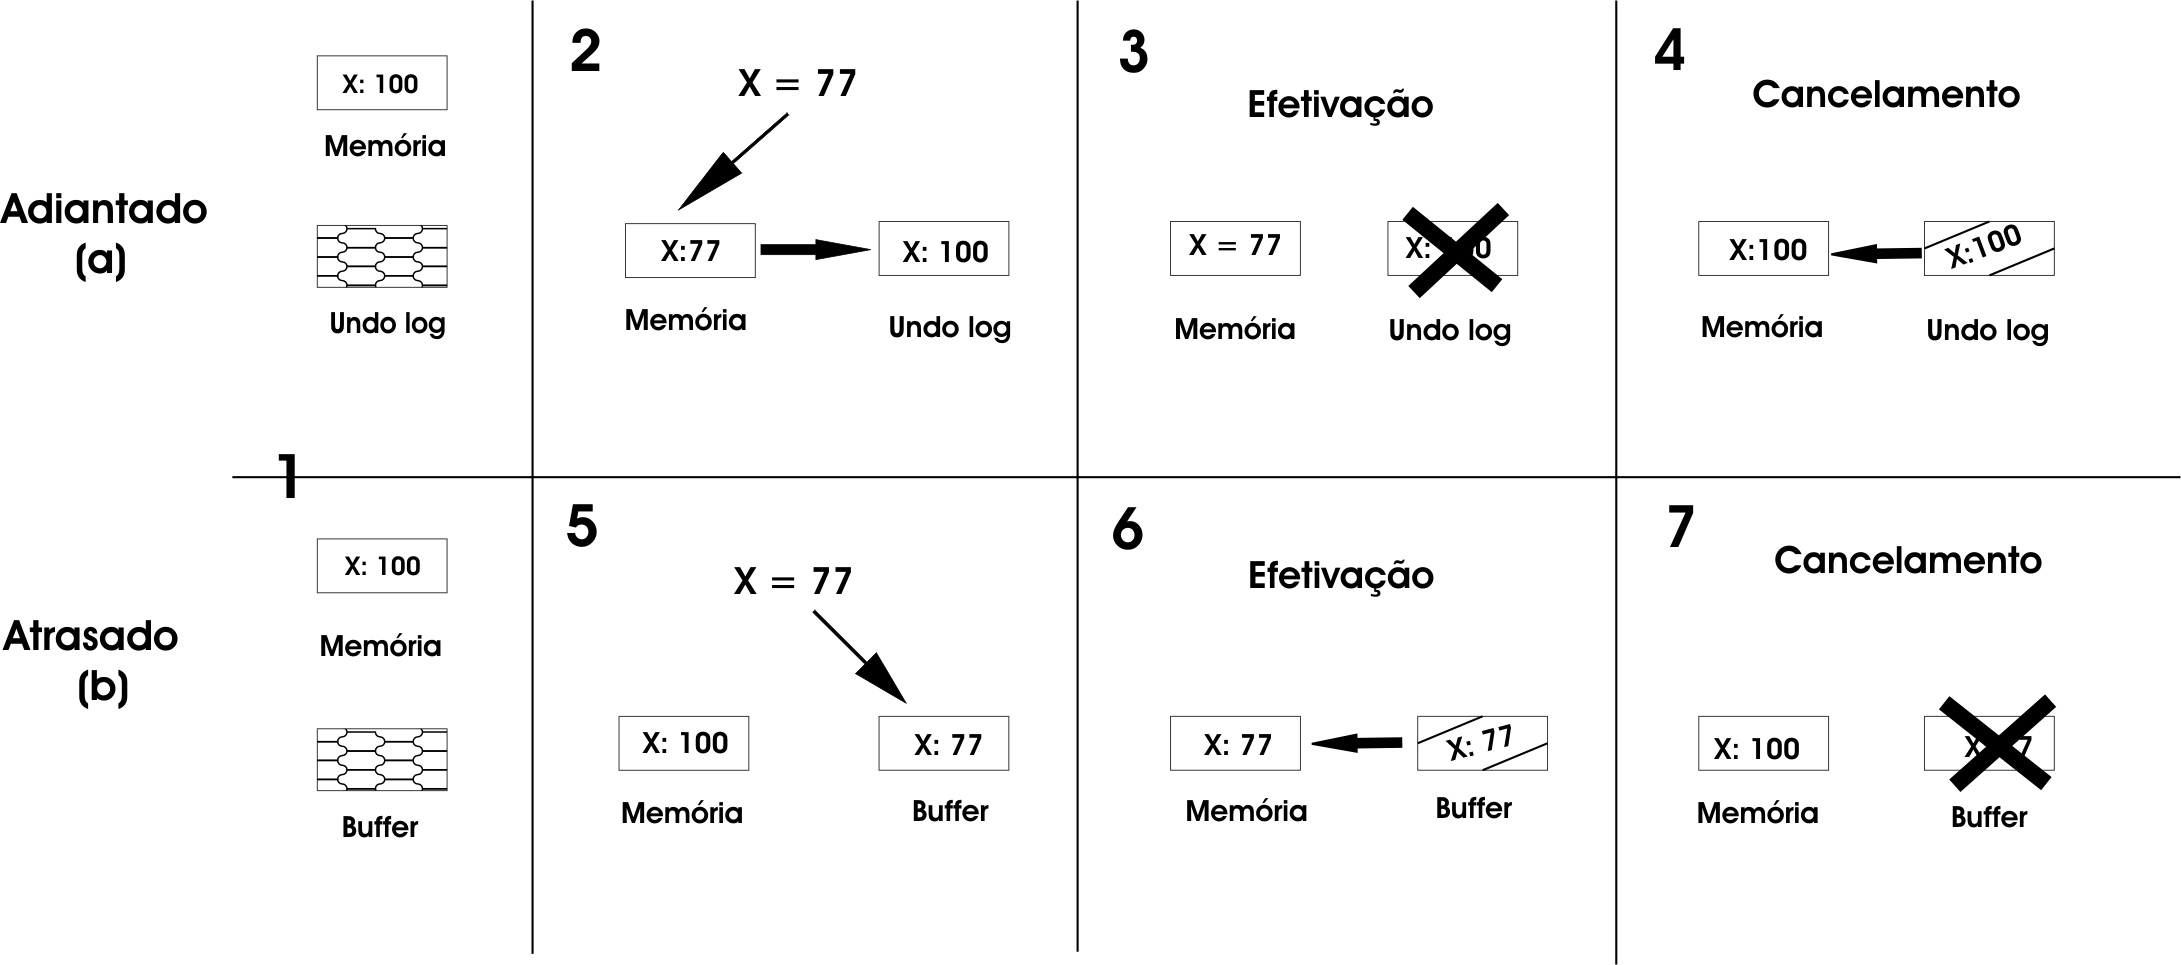
\includegraphics[height=7cm]{images/versionamento.png}
\caption{Exemplo de versionamento adiantado (a) e atrasado (b). Fonte:~\cite{BaldassinTese2009}}
\label{figuraversionamento}
\end{figure}

Existem dois tipos de versionamento de dados:

\begin{itemize}
 \item \textbf{Versionamento Adiantado}: como pode ser visto na Figura~\ref{figuraversionamento}~(a), o valor modificado durante a transação é armazenado direto na memória e o valor inicial é armazenado em um \emph{undo log}, para que no caso de cancelamento na transação o valor inicial seja restaurado na memória.

 \item \textbf{Versionamento Atrasado}: como pode ser visto na Figura~\ref{figuraversionamento}~(b) neste versionamento o valor modificado durante a transação é armazenado em um \emph{buffer} e o valor inicial é mantido na memória até que aconteça um \emph{commit} na transação, onde o valor armazenado no \emph{buffer} é escrito na memória. Caso aconteça o cancelamento na transação, o valor do \emph{buffer} é descartado.
\end{itemize}

\section{Detecção de Conflito}

Mecanismos de detecção de conflitos verificam a existência de operações conflitantes durante uma transação. Um conflito ocorre quando duas transações estão acessando um mesmo dado na memória e pelo menos uma das transações está fazendo uma operação de escrita~\cite{BaldassinTese2009}.

Da mesma forma que o versionamento de dados, a detecção de conflito também pode ser de dois tipos:

\begin{itemize}
 \item \textbf{Detecção de Conflitos Adiantado}: ocorrem no momento em que duas transações acessam um mesmo dado e uma delas faz uma operação de escrita. Essa operação de escrita é detectada e então uma transação é abortada. Neste tipo de detecção pode ocorrer um problema chamado de \emph{livelock}, quando duas transações ficam cancelando-se, desta forma, a execução do programa não progride. A Figura~\ref{figuradeteccaoadiantado} mostra como é feita a detecção de conflitos adiantado.

 O Caso~1, mostra a execução sem conflitos, onde as duas transações são executadas sem problemas. Já o Caso~2, mostra o que acontece quando ocorre um conflito, onde T1 lê A e logo depois T2 escreve em A, então o conflito é detectado e T1 é abortada, após ser efetivada T2, a transação T1 consegue ler A sem problema de conflito. Por fim o Caso~3 mostra a situação de \emph{livelock}, onde as duas transações tentam ler e escrever em A, assim as duas acabam sempre se abortando.

\begin{figure}[!htp]
\centering
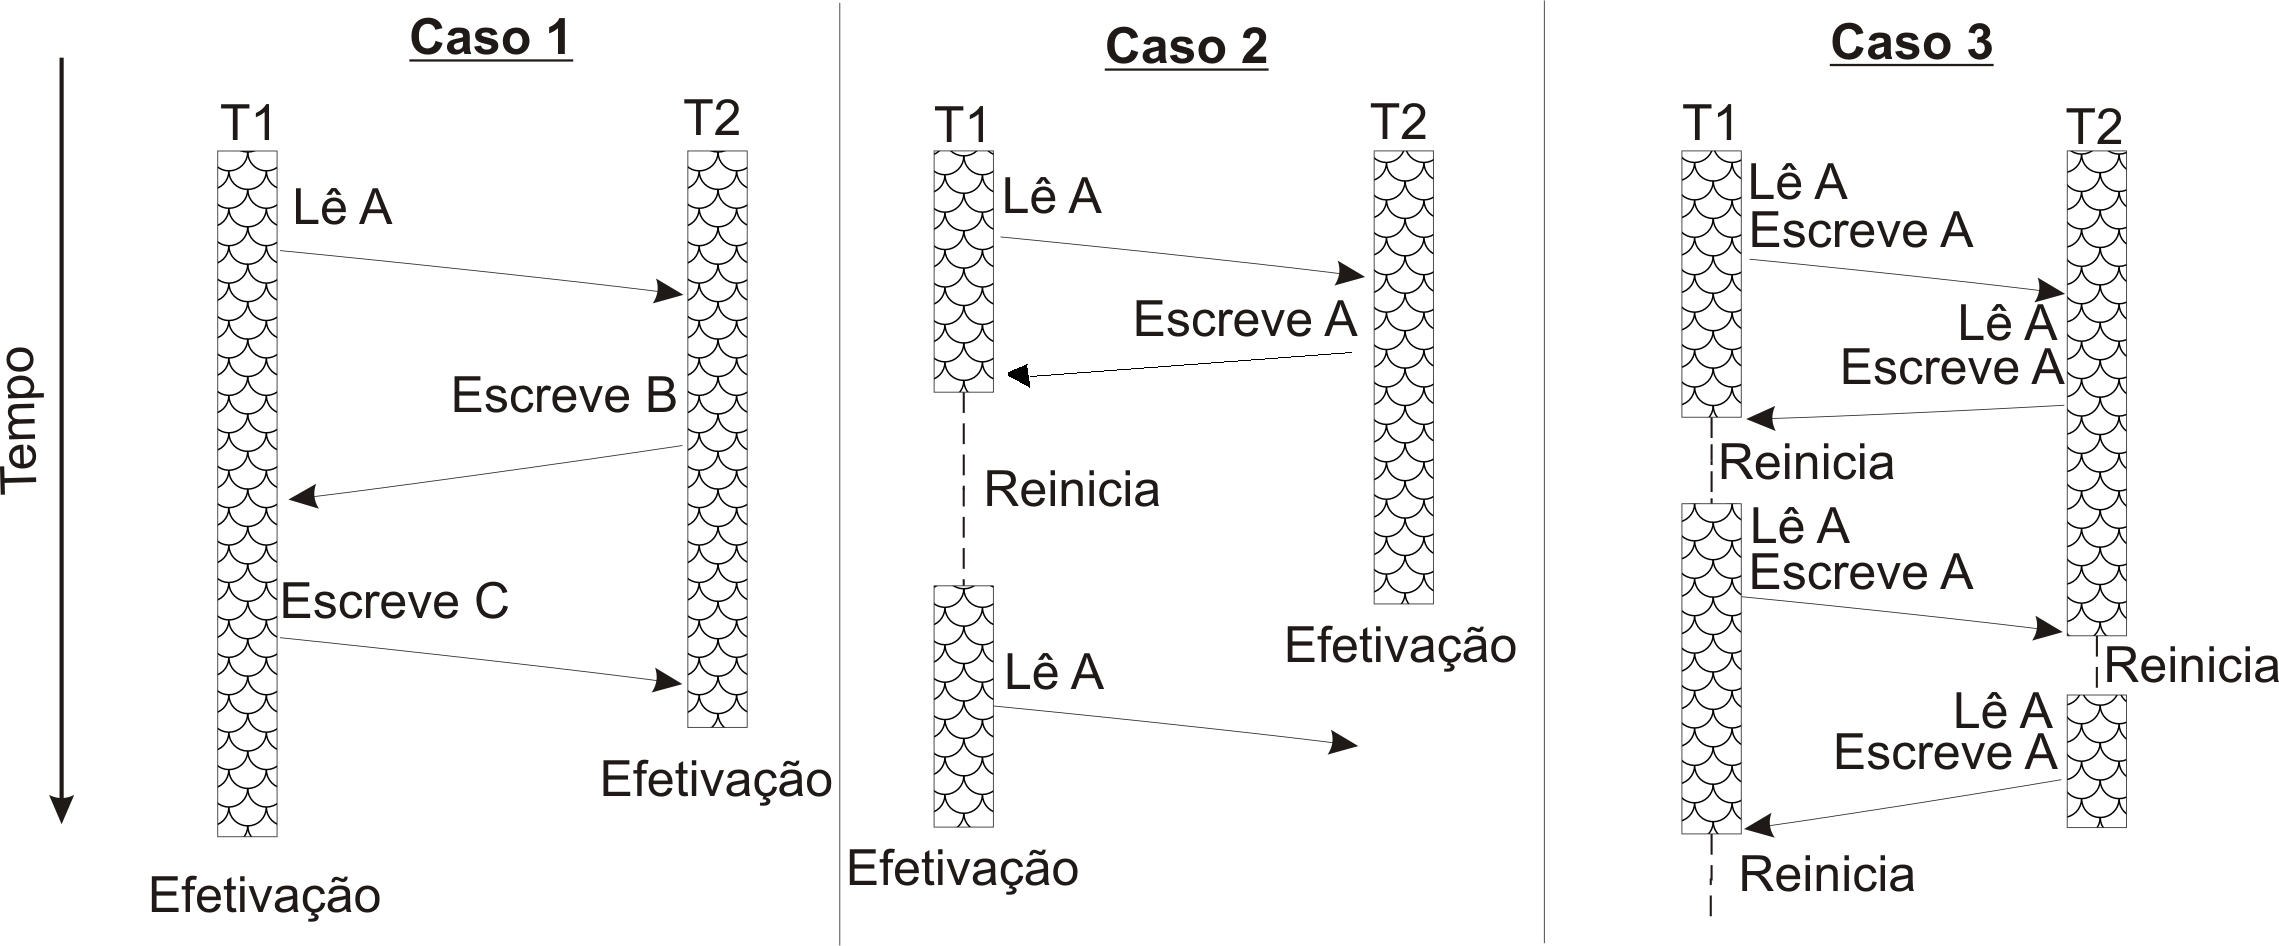
\includegraphics[height=6.5cm]{images/conflitoadiantado.png}
\caption{Detecção de conflitos em modo adiantado. Fonte:~\cite{rigotm}}
\label{figuradeteccaoadiantado}
\end{figure}


 \item \textbf{Detecção de Conflitos Atrasado}: Este tipo de detecção de conflito ocorre no final da transação.  Antes da transação ser efetuada, é verificado se ocorreu um conflito. Caso tenha ocorrido, a transação é cancelada, senão é efetivada. Para transações muito grandes não é recomendado este tipo de detecção, pois uma transação grande pode ser abortada várias vezes por transações pequenas, assim gastando tempo de processamento desnecessário, este problema se chama \emph{starvation}. A Figura~\ref{figuradeteccaoatrasado} mostra como é feita a detecção de conflitos atrasado.

 O Caso~1, mostra as transações acessando dados diferentes, não ocasionando conflitos. No Caso~2, T2 lê A que é escrita por T1. A T2 só nota o conflito quando T1 é efetivado. Logo depois de notar o conflito T2 é abortada. No Caso~3 não ocorre nenhum conflito, pois T1 lê A antes de T2 escrever. O Caso~4 mostra a situação em que, após ser cancelada, T1 volta a executar.
\end{itemize}

\begin{figure}[!htp]
\centering
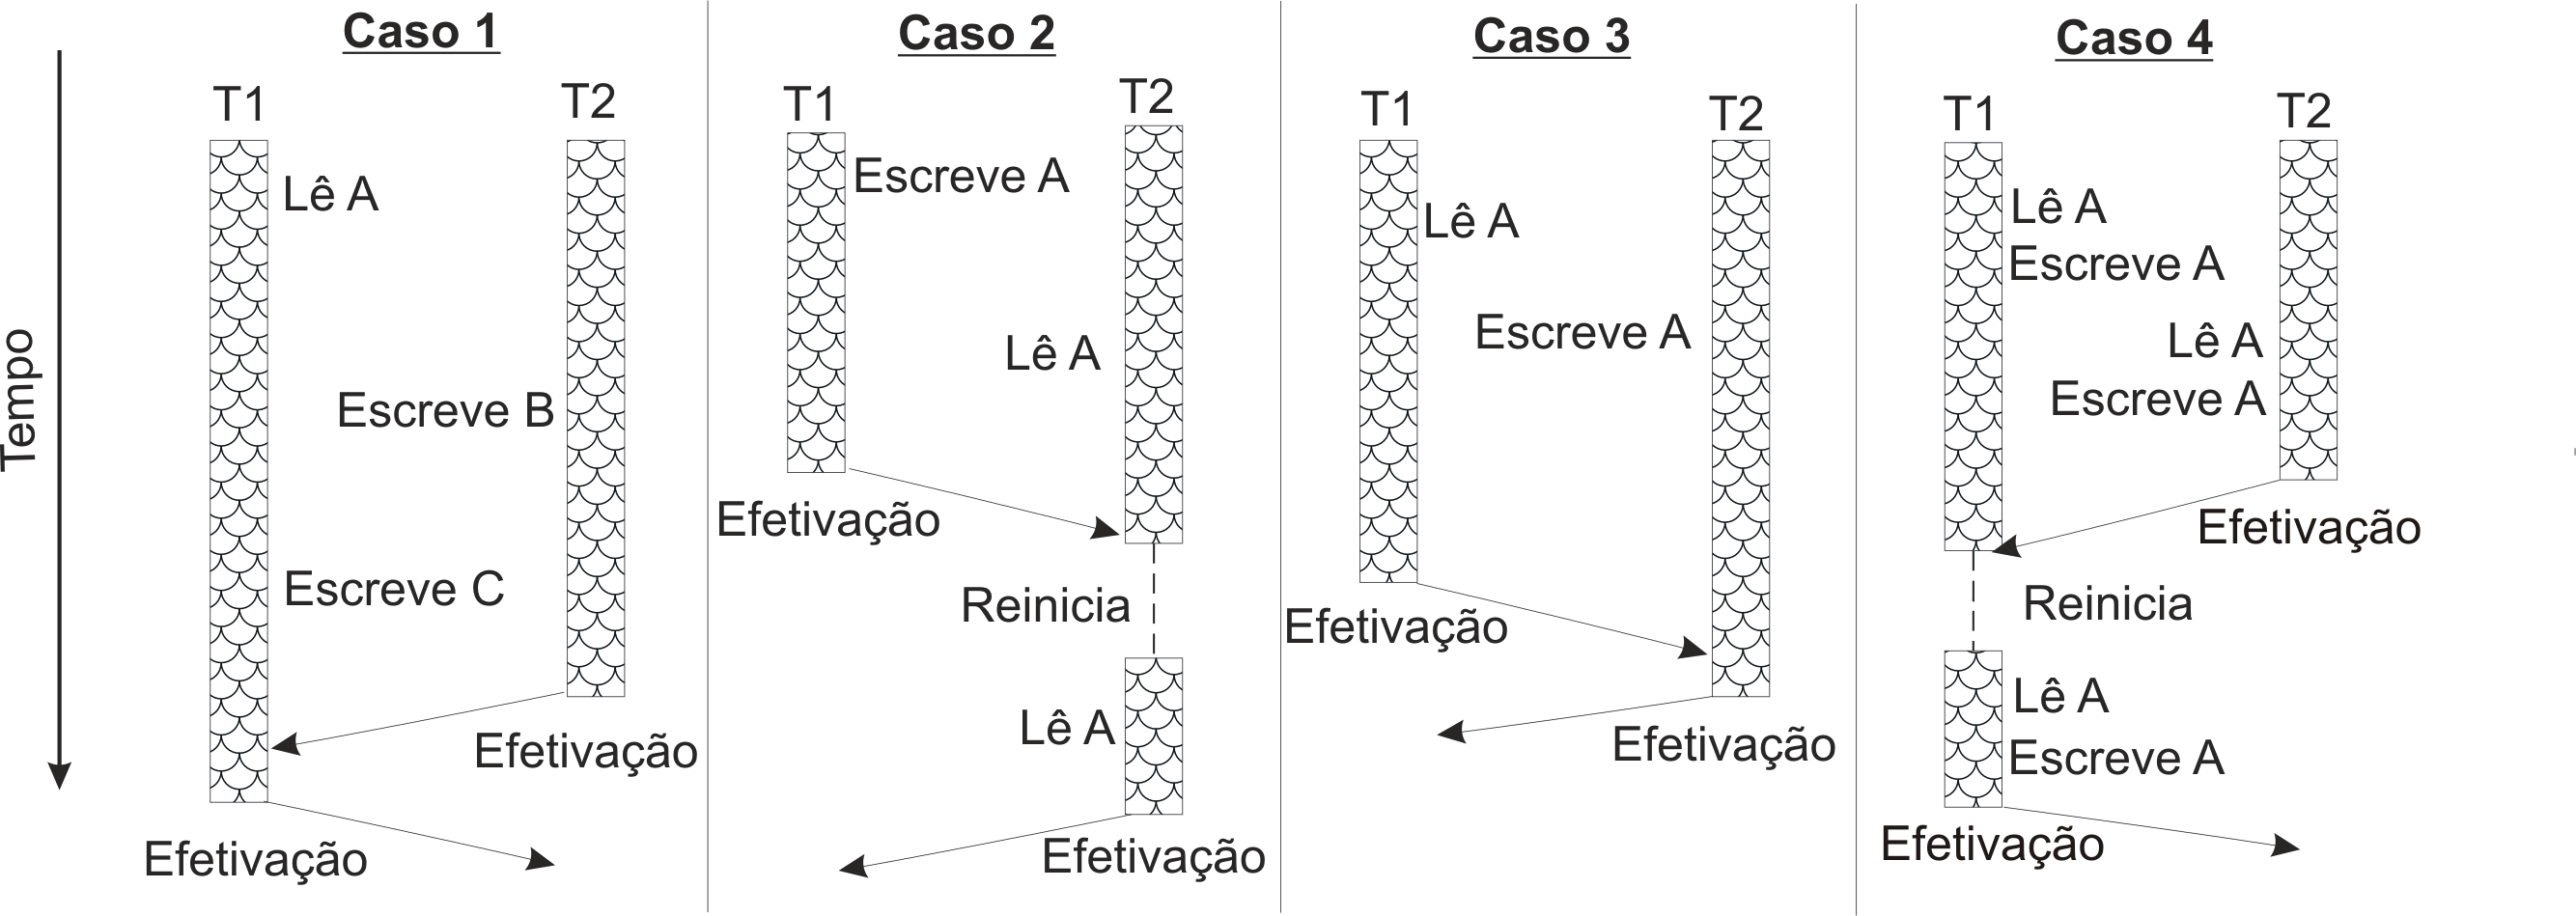
\includegraphics[height=6.5cm]{images/conflitoatrasado.png}
\caption{Detecção de conflitos em modo atrasado. Fonte:~\cite{rigotm}}
\label{figuradeteccaoatrasado}
\end{figure}


Para solucionar o problema de qual transação continuará executando, quando ocorre um conflito, é utilizado um gerenciador de contenção~\cite{TM2010}. O gerenciador de contenção é o responsável por decidir quando e qual transação vai ser abortada, isso para garantir que a execução do programa prossiga sem problemas.

\section{TinySTM}

A \emph{TinySTM}~\cite{TINY} é uma implementação de STM para as linguagens C e C++. Seu algoritmo é baseado em outros algoritmos de STM como o TL2~(\emph{Transactional Locking} 2)~\cite{tl2}. Ela é uma biblioteca utilizada para escrever aplicativos que usam memórias transacionais para sincronização, em substituição aos tradicionais \emph{locks}.

\subsection{Sincronização e Versionamento}

Na \emph{TinySTM} a sincronização é feita a partir de um \emph{array} de \emph{locks} compartilhado que gerencia o acesso concorrente à memória. Cada \emph{lock} é do tamanho de um endereço da arquitetura~\cite{TINY}, e bloqueia vários endereços de memória. O mapeamento é feito por meio de uma função \emph{hash}. A Figura~\ref{figurasincronisacaotinystm} apresenta as estruturas de dados utilizadas nesta implementação.

\begin{figure}[!htp]
\centering
\includegraphics[height=8cm]{images/tinystm.png}
\caption{Estruturas de dados utilizadas na \emph{TinySTM}. Fonte:~\cite{TINY}}
\label{figurasincronisacaotinystm}
\end{figure}

O bit menos significativo é utilizado para indicar se o \emph{lock} está em uso. Se o bit menos significativo indicar que o \emph{lock} não está em uso, nos bits restantes são armazenados um número de versão que corresponde ao \emph{timestamp} da transação que escreveu por último em um dos locais de memória abrangidos pelo \emph{lock}.

Se o bit menos significativo indica que o \emph{lock} está em uso, então nos bits restantes é armazenado um endereço que identifica a transação que está utilizando o dado~(isso utilizando o versionamento adiantado), ou uma entrada no \emph{write set} da transação que está utilizando o dado~(isso utilizando o versionamento atrasado). Em ambos os casos os endereços apontam para uma estrutura que é \emph{word-aligned} e seu bit menos significativo é sempre zero, por isso, o bit menos significativo pode ser utilizado como bit de bloqueio.

Quando utilizado o versionamento atrasado, o endereço armazenado no \emph{lock} permite uma operação rápida para localizar as posições de memória atualizadas abrangidas pelo \emph{lock}, no caso de serem acessados novamente pela mesma transação. Em contraste, a TL2 deve verificar o acesso à memória se a transação atual ainda não escreveu neste endereço, o que pode ser caro quando \emph{write sets} são grandes. A leitura depois da escrita não é um problema quando é utilizado o versionamento adiantado porque a memória sempre contém o último valor escrito na memória pela transação ativa.

A \emph{tinySTM} apresenta três estratégias de versionamento distintas que podem ser utilizadas, sendo que duas utilizam versionamento atrasado~(write-back) e uma utiliza versionamento adiantado~(write-through), estas são:

\begin{itemize}
 \item \textbf{Write\_Back\_ETL}: esta estratégia implementa o versionamento atrasado com \emph{encounter-time locking}, isso é, o \emph{lock} é adquirido após ocorrer uma operação de escrita e atualiza o \emph{buffer}. O valor é escrito na memória no momento do \emph{commit} da transação;

 \item \textbf{Write\_Back\_CTL}: esta estratégia implementa o versionamento atrasado com \emph{commit-time locking},isto é, ele adquire o \emph{lock} antes de ocorrer o um \emph{commit} e atualizar o \emph{buffer}. Assim como no \emph{Write-Back-ETL} o valor é escrito na memória no momento do \emph{commit} da transação;

 \item \textbf{Write\_Through}: esta estratégia implementa o versionamento adiantado com \emph{encounter-time locking}, isto é, o valor é escrito direto na memória e mantém um \emph{undo log}, caso ocorra um \emph{abort} na transação é possível restaurar o valor anterior na memória.
\end{itemize}

A \emph{TinySTM} utiliza \emph{Write\_Back\_ETL} como sua estratégia de versionamento padrão.

\subsection{Escritas}

Quando ocorre uma escrita em um local da memória, a transação primeiro identifica o \emph{lock} correspondente ao endereço de memória e lê o valor. Se o \emph{lock} está em uso a transação verifica se é a proprietária do \emph{lock} utilizando o endereço armazenado nos restantes bits de entrada. Caso a transação seja a proprietária então ela simplesmente escreve o novo valor e retorna. Caso contrário, a transação pode esperar por algum tempo ou abortar imediatamente. A \emph{TinySTM} utiliza a última opção como padrão em sua implementação.

Se o \emph{lock} não está em uso, a transação tenta adquiri-lo para escrever o novo valor na entrada utilizando uma operação atômica \emph{compare-and-swap}. A falha indica que outra transação adquiriu o \emph{lock} nesse meio tempo, então a transação é reiniciada.


\subsection{Leituras}

Quando ocorre uma leitura na memória, a transação deve verificar se o \emph{lock} está em uso ou se  o valor já foi atualizado concorrentemente por outra transação. Para esse fim, a transação lê o \emph{lock} correspondente ao endereço de memória. Se o \emph{lock} não tem proprietário e o valor~(número de versão) não foi modificado entre duas leituras, então o valor é consistente.

\subsection{Gerenciamento de Memória}

A \emph{TinySTM} utiliza um gerenciador de memória que possibilita qualquer código transacional utilizar memória dinâmica. As transações mantém o endereço da memória alocada ou liberada. A alocação de memória é automaticamente desfeita quando a transação é abortada, já a liberação não pode ser desfeita antes do \emph{commit}. Contudo uma transação pode somente liberar memória depois de adquirir todos os \emph{locks}, assim, um \emph{free} é semanticamente equivalente a uma atualização.

\subsection{Gerenciador de Contenção}

A \emph{TinySTM} implementa quatro estratégias de gerenciador de contenção, estas são:

\begin{itemize}
 \item \textbf{CM\_Suicide}: nesta estratégia a transação que detecta o conflito é abortada imediatamente;

 \item \textbf{CM\_Delay}: esta estratégia assemelhasse a \emph{CM\_Suicide}, porem, espera até que a transação que gerou o \emph{abort} tenha liberado o \emph{lock}, então reinicia a transação. Isto porque por intuição a transação a transação que foi abortada irá tentar adquirir o mesmo \emph{lock} novamente, provavelmente falhando em mais de uma tentativa. Está estratégia aumenta as chances de que a transação tenha sucesso sem gerar um grande número de \emph{aborts}, melhorando o tempo de execução do processador;

 \item \textbf{CM\_Backoff}: também parecida com a \emph{CM\_Suicide}, esta estratégia espera um tempo randômico para reiniciar a transação. Este tempo de espera é escolhido ao uniformemente ao acaso em um intervalo cujo tamanho aumenta exponencialmente a cada reinicialização;

 \item \textbf{CM\_Modular}: esta estratégia implementa vários gerenciadores de contenção, que são alternados durante a execução. Os gerenciadores utilizados são:

    \begin{itemize}
       \item \textbf{Suicide}: a transação que descobriu o conflito é abortada;

       \item \textbf{Aggressive}: é o inverso da \emph{Suicide}, a transação abortada é a outra e não a que descobriu o conflito;

       \item \textbf{Delay}: a mesma que a \emph{Suicide}, mas aguarda pela resolução do conflito para reiniciar a transação;

       \item \textbf{Timestamp}: a transação mais nova é abortada.
    \end{itemize}

\end{itemize}

A \emph{TinySTM} utiliza a \emph{CM\_Suicide} como sua estratégia padrão de gerenciamento de contenção.

\section{STAMP}
\label{section:stamp}


\emph{Stanford Transactional Applications for Multi-Processing}~\cite{STAMP} é um conjunto de \emph{benchmarks} criado para pesquisa de memórias transacionais, composto por oito \emph{benchmarks}. Apesar de desenvolvido para a STM~TL2, com algumas modificações disponíveis pode ser usado no \emph{TinySTM}.

%A versão do STAMP utilizada será a 0.9.10.
% O conjunto de \emph{benchmarks} STAMP foi escolhido devido a ele implementar vários \emph{benchmarks}, assim, atingindo uma maior área de aplicações das STM além de ser o conjunto de \emph{benchmark} mais utilizado na pesquisa de STM.

O conjunto de \emph{benchmarks} STAMP implementa vários \emph{benchmarks}, assim, atingindo uma maior área de aplicações das STM e é o conjunto de \emph{benchmark} mais utilizado na pesquisa de STM. Os oito benchmarks apresentados são:

\begin{itemize}
  \item \textbf{Bayes}: Apresenta uma rede bayesinana de aprendizado;
  \item \textbf{Genome}: Implementa uma aplicação que reconstrói a sequencia de um gene a partir de sequências maiores;
  S\item \textbf{Intruder}: Simula o Design 5 do \emph{Network Intrusion Detection System}~(NIDS)~\cite{Haagdorens05};
  \item \textbf{Kmeans}:  \emph{K-means} é um algoritmo comumente usado para partição de itens de dados em subconjuntos relacionados;
  \item \textbf{Labyrinth}: Implementa uma algoritmo que descobre o menor caminho entre um ponto inicial e um ponto final;
  \item \textbf{SSCA2}: É composto por quatro \emph{kernels} que operam em um grande, dirigido e ponderado gráfico;
  \item \textbf{Vacation}: Implementa um sistema de reserva de viagens alimentado por um banco de dados não-distribuído; e
  \item \textbf{Yada}: Implementa o algoritmo de Ruppert~\cite{Ruppert95} para refinamento de malha.
\end{itemize}

Neste trabalho vai ser utilizada a versão 0.9.10 do STAMP para avaliar e comparar a execução da biblioteca de STM TinySTM atual e a utilização do escalonador proposto.

% Os \emph{benchmarks} implementados pelo STAMP são~\cite{STAMP}:
% \newline


% \subsection{Bayes}

% Esta aplicação implementa um algoritmo de aprendizado de redes Bayesianas, que é uma parte importante do aprendizado de máquina. Normalmente, nem as distribuições de probabilidades nem as dependências condicionais entre eles são conhecidas ou podem ser resolvidos por um ser humano, assim redes Bayesianas são frequentemente estudadas com os dados observados. O algoritmo específico implementa uma estratégia de \emph{hill-climbing} ou subida de encosta que usa buscas locais e globais, semelhante à técnica descrita em~\cite{bayesian}. Para estimativas eficientes de distribuição de probabilidade, utiliza-se uma \emph{adtree} ou árvore de decisão a partir de~\cite{Moore97}.


% \subsection{Genome}

% Este \emph{benchmark} implementa um programa de sequenciamento de genes que reconstrói a sequência de genes a partir de sequências maiores. O algoritmo usado para o sequenciamento de genes têm  três fases:

% \begin{enumerate}
%   \item [1.] Remove os segmentos duplicados utilizando uma \emph{hash};
%   \item [2.] Combina segmentos utilizando o algoritmo de pesquisa de sequência \emph{Rabin-Karp}~\cite{Karp87}; e
%   \item [3.] Constrói a sequência.
%   \newline
% \end{enumerate}


% \subsection{Intruder}

% Este \emph{benchmark} simula o Design 5 dos NIDS~(\emph{Network Intrusion Detection System}) descritos por Haagdorens em~\cite{Haagdorens05}. Pacotes de rede são processados paralelamente e passam por três fases: captação, remontagem e detecção. A estrutura de dados principal na fase de captura é uma simples fila, e a fase de remontagem utiliza um dicionário (implementado por uma árvore auto balanceada), que contém a lista de pacotes que pertencem à mesma seção. Ao avaliar seus cinco designs para um NIDS \emph{multithread}, Haagdorens afirma que a complexidade da fase de remontagem fez com que ele utilize a sincronização de grãos grosso nos designs~4 e~5. Assim, embora estes dois modelos tentam explorar níveis mais elevados de simultaneidade, a sincronização aproximada de grão resulta em um pior desempenho.


% \subsection{Kmeans}

% Este \emph{benchmark} foi tirado do \emph{NU-MineBench 2.0}~\cite{Pisharath05}. \emph{K-means} é um método baseado em partição~\cite{Bezdek81} e é sem dúvida a técnica de agrupamento mais utilizada. Este algoritmo é comumente usado para partição de itens de dados em subconjuntos relacionados. Cada \emph{thread} processa uma partição dos objetos iterativamente. A versão transacional adiciona uma transação para proteger o update do centro do \emph{cluster} que ocorre durante cada iteração.


% \subsection{Labyrinth}

% Dado um labirinto, este \emph{benchmark} encontra os caminhos de menor distância entre os pares de pontos inicial e final. O algoritmo de roteamento utilizado é o algoritmo Lee~\cite{Lee61}.

% Nesse algoritmo, o labirinto é representado como uma grade, em que cada ponto de grade pode conter ligações adjacentes, para os pontos da grade que não estão nas diagonais. O algoritmo busca um caminho mais curto entre os pontos de conexão através da realização de uma busca em largura e marca cada ponto da grade com a sua distância para o início. Esta fase de expansão acabará por chegar ao ponto final, se a conexão for possível. A segunda fase de rastreamento, em seguida, estabelece a ligação, seguindo todo o caminho diminuindo a distância. Este algoritmo é garantido para encontrar o caminho mais curto entre um ponto inicial e final, no entanto, quando vários caminhos são feitos, um caminho pode bloquear outro.


% \subsection{SSCA2}

% \emph{Scalable Synthetic Compact Applications 2}~(SSCA2)~\cite{Bader05} é composta por quatro \emph{kernels} que operam em um grande, dirigido e ponderado gráfico. Estes quatro \emph{kernels} gráficos são comumente usados em aplicações que vão desde a biologia computacional até a segurança. STAMP incide sobre um \emph{Kernel}, que constrói uma estrutura de dados eficiente utilizando matrizes de adjacência e matrizes auxiliares.


% \subsection{Vacation}

% Este \emph{benchmark} implementa um sistema de reserva de viagens alimentado por um banco de dados não-distribuído. A carga de trabalho é composto por vários segmentos de clientes que interagem com o banco de dados via gerenciador de transações do sistema.

% O banco de dados é composto por quatro tabelas: carros, quartos, voos e clientes. Os três primeiros têm relações com os campos que representam um número único de identificação, quantidade reservada, a quantidade total disponível, e preço. A tabela de clientes acompanha as reservas feitas por cada cliente e o preço total das reservas que eles fizeram. As tabelas são implementados como árvores rubro negras.


% \subsection{Yada}

% Este \emph{benchmark} implementa o algoritmo de Ruppert para refinamento de malha~\cite{Ruppert95}. A versão transacional é similar em design ao apresentado em~\cite{Kulkarni06}.

% \subsection{Biblioteca Thread.h}

% O conjunto de \emph{benchmark} STAMP disponibiliza para os \emph{benchmarks} a biblioteca de \emph{threads} \emph{thread.h}. Esta dispõem do mecanismo \emph{pthread} e \emph{thread\_barrier} para criar um \emph{pull} de trabalhos a ser executado.

% A biblioteca dispõem de uma \emph{struct} \emph{thread\_barrier\_t} e disponibiliza as seguintes funções:

% \begin{itemize}

% \item thread\_startup;
% \item thread\_start;
% \item thread\_shutdown;
% \item thread\_barrier\_alloc;
% \item thread\_barrier\_free;
% \item thread\_barrier\_init;
% \item thread\_barrier;
% \item thread\_getId;
% \item thread\_getNumThread; e
% \item thread\_barrier\_wait.

% \end{itemize}

% As funções apresentadas acima manipulam a \emph{struct}, Figura~\ref{fig:struct}, disponível na biblioteca provendo a execução do \emph{pool} de trabalhos.

% \begin{figure}[!ht] 
%   \centering
%   \begin{verbatim}
%                     typedef struct thread_barrier {
%                         THREAD_MUTEX_T countLock;
%                         THREAD_COND_T proceedCond;
%                         THREAD_COND_T proceedAllCond;
%                         long count;
%                         long numThread;
%                     } thread_barrier_t;
%   \end{verbatim}
%   \caption{Struct disponível na thread.h do \emph{benchmark STAMP}}
% \label{fig:struct}
% \end{figure}

% A função \emph{threadWait} disponível em \emph{thread.c} realiza a sincronização de todas as \emph{threads} disponíveis no \emph{pool} de \emph{thread}. \emph{thread\_startup} recebe como parâmetro o número de \emph{threads} a ser criado e realiza a inicialização do \emph{pool} de \emph{threads}.

% A função \emph{thread\_start} executa as \emph{threads} disponíveis no \emph{pool de thread} utilizando uma chamada de função para \emph{threadWait}. A partir desta função são executadas as tarefas e utilizadas as demais funções. A biblioteca de escalonamento desenvolvida neste trabalho, tem como base as funções básicas citadas acima.

\chapter{Escalonadores}
\label{chapter::escalonadores}

O uso de escalonadores provem melhorias nas execuções de programas, pode-se utilizar escalonadores de tarefas para melhorar o desempenho de arquiteturas, como visto no trabalho \cite{Rodolfo:2014}, consegue-se utilizar um escalonador para reduzir a latência de acesso à memória pelo processador em arquiteturas \emph{NUMA}.

Em STM o uso de escalonadores pode reduzir o número de conflitos gerados pelo aumento do paralelismo, como podemos ver em \cite{Nicacio2012} o \emph{LUTS} apresenta heurísticas de detecção de conflitos para que o escalonador de transações evite \emph{aborts} no decorrer de sua execução.

%\section{Heurísticas}

Escalonadores fornecem diferentes abordagens para cada problema proposto, estas distintas abordagens permitem aos desenvolvedores explorar heurísticas de escalonamento que se adaptam a arquitetura utilizada propiciando uma solução mais eficiente.

Existem muitas heurísticas diferentes para prever conflitos, estas podem servir como base para o escalonamento de transações. Para este trabalho foram estudados algumas das principais heurísticas e suas classificações.

O trabalho apresentado em~\cite{disanzo2017} fornece uma categorização dos escalonadores de STM, na qual os algoritmos são classificados de acordo com suas heurísticas.

Está categorização é dividida em algoritmos Baseados em Heurística e algoritmos Baseados em Modelo. Cada categorização possui classificações de acordo com o comportamento de sua heurística.

\begin{itemize}
	\item Baseado em Heurística:
	\begin{itemize}
	    \item Feedback: Utiliza o feedback da execução para realimentar sua heurística;
	    \item Predição: Utiliza uma predição das informações para tomada de decisão;
	    \item Reativo: Só executa sua heurística após determinado comportamento da aplicação ocorrer; e
	    \item Heurística Mista: Mescla as classificações anteriores para otimizar a heurística.
	\end{itemize}
	\item Baseado em Modelo:
	\begin{itemize}
	    \item Aprendizado de Máquina: Utiliza algoritmos de aprendizado de máquina para tomar decisão;
	    \item Modelo Analítico: Monta modelos analíticos para tomar decisão; e
	    \item Modelo Misto: Mistura as classificações acima para otimizar a heurística.
	\end{itemize}
\end{itemize}


% \section{Categorias}

A tabela~\ref{tab:compare} apresenta as classificações dos principais algoritmos revisados na bibliografia durante o desenvolvimento deste trabalho.

\begin{table}[]
\footnotesize
\centering
\caption{Algoritmos e técnicas de escalonamento}
\label{tab:compare}
\begin{tabular}{l|l}
\hline
Escalonador & Técnica \\ \hline
ATS & Feedback \\
Probe & Feedback \\
F2C2 & Feedback \\
Shrink & Predição \\
SCA & Predição \\
CAR-STM & Reativo \\
RelSTM & Reativo \\
LUTS & Heurística Mista \\
ProVIT & Heurística Mista \\
SAC-STM & Aprendizado de Máquina \\
CSR-STM & Modelo Analítico \\
MCATS & Modelo Analítico \\
AML & Modelo Misto \\
\hline
\end{tabular}
\end{table}

\section{ATS}

\emph{Adaptive Transaction Scheduling}~(ATS)~\cite{ats2008} foi um dos primeiros trabalho a apresentar um escalonador de MT para trabalhar junto com gerenciador de contenção.

O ATS utiliza um valor para tomada de decisão denominado CI (Contention Intensity), cada thread em execução possui seu próprio CI. O CI é calculado cada vez que ocorre um commit ou um abort e é zerado a cada inicio de transação.

O escalonador utiliza o valor do CI em sua tomada de decisão. Quando o valor do CI ultrapassa um limiar pré definido, a thread é colocada em uma única fila para garantir uma execução de forma serial.

\section{CAR-STM}

\emph{Collision Avoidance and Resolution}~(CAR-STM)~\cite{carstm2008} foi desenvolvido para evitar que conflitos já existentes voltem a ocorrer. Para isto é apresentado duas heurísticas de gerenciamento.

A primeira heurística é denominada Básica e busca executar de forma serial as transações conflitantes sem manter um histórico da execução. A segunda denominada Permanente busca manter um histórico das transações que conflitaram e executa-las de forma serial.

\begin{itemize}
  \item Básica: Quando detectado um conflito, a transação mais recente é abortada e migrada para fila da transação conflitante, assim sua execução sera serializada.
  \item Permanente: Quando uma transação Tb aborta em relação a Ta, Tb é migrado para fila de Ta e sua ordem de execução será Ta -> Tb. Caso a transação Ta conflite e aborte em relação a Tc, Ta deverá ser migrada para fila de Tc carregando sua dependência Ta -> Tb.
\end{itemize}

\section{LUTS}

\emph{Light-Weight User-Level Transaction Scheduler}~(LUTS)~\cite{Nicacio2012} apresenta um escalonador que busca evitar a ociosidade de um núcleo após a serialização de uma transação. 

Para isto cada thread é representado internamente por um Registro de Contexto em Execução (RCE), cada RCE encapsula uma thread. No inicio da execução o escalonador cria uma fila de RCEs para serem executados no futuro.

Assim o LUTS dispara um RCE por núcleo, e utiliza a fila para não disparar mais RCEs que núcleos disponíveis. Cada REC disparado é convertido em uma thread de sistema que executa um conjunto de transações.

Na tentativa de evitar conflitos o LUTS apresenta uma forma dinâmica para soluciona-los, considerando transações curtas e transações longas. Para definir o tamanho da transação é utilizada a contagem de ciclos da mesma, onde a partir de 100 mil ciclos temos uma transação longa.

Para transações curtas, a heurística utilizada é similar a do ATS, o escalonador calcula a intensidade de conflito da transação e serializa esta quando o calculo ultrapassa um limiar. Porém o LUTS escolhe outra transação para substituir a atual.

Para transações longas, a heurística é mais elaborada, utilizando três metadados globais:

\begin{itemize}
  \item  activeTx: Um vetor de tamanho igual ao total de núcleos disponíveis, usado para armazenar o identificador da transação que está sendo executada.
  \item conflictTable: Uma tabela do histórico de conflitos, cada linha armazena um conjunto de transações dada pelo activeTx, e cada coluna armazena a probabilidade de conflito.
  \item bestTx: Um vetor que sumariza a melhor transação a ser executada para cada núcleo.
\end{itemize}

Quando uma transação realiza um commit ou abort o escalonador se encarrega de atualizar a conflictTable na sua respectiva linha, aumentando ou diminuindo sua probabilidade de conflito.

Para evitar percorrer a conflictTable no inicio de cada transação o LUTS percorre a bestTx e seleciona qual transação deve executar. Quando a conflictTable é atualizada o escalonador atualiza a bestTx.

\section{Shirink}

\emph{Shirink}~\cite{shirink2009} apresenta um escalonador que busca minimizar a ocorrência de aborts com base nos conjuntos de leituras e escritas ocorridos em cada thread.

O escalonador é baseado em predição e usa como heurística os acessos à memória das transações executadas anteriormente. Para evitar overhead em sua execução o Shirink avalia os acessos apenas se existir uma alta contenção no sistema.

No inicio de cada transação o escalonador avalia se existe a relação entre commit e abort é superior a um limiar predefinido, se esse valor for superior ao limiar o escalonador considera que o sistema possui uma alta contenção e ativa a heurística para serializar as transações em execução.

Cada thread possui um conjunto dos acessos de leitura e escrita realizados pelas transações, quando uma transação vai iniciar com um sistema de alta contenção esse conjunto de leitura e escrita é verificado, se outra thread em execução possuir um conjunto semelhante o escalonador assume que há uma alta chance da transação abortar.

Para que a transação não aborte a thread que iniciaria a transação é bloqueada até o fim da transação na thread em execução, assim o Shrink busca forçar a serialização das execuções.

\section{ProVit}

O escalonador \emph{ProVIT}~\cite{rito2015} fornece uma abordagem otimista da execução, evitando considerar que toda transação que abortou ira abortar novamente na sequencia. 

Assim como o LUTS o ProVIT avalia o tamanho das operações atômicas para aplicar sua heurística. Porém no ProVIT mais de uma heurística pode estar ativa ao mesmo tempo. 

Também foi apresentada a observação que duas transações conflitantes, de leitura e escrita, podem efetuar o commit dependendo da ordem, se o commit for efetuado primeiro pela transação de leitura, a de escrita não será conflitante.

Operações atômicas longas utilizam uma política é baseada em grão fino para melhorar a precisão da predição e evitar a reexecução de transações. Essa predição utiliza como base o conjunto de leitura das transações já executadas.

Se uma transação efetua um abort o escalonador marca esta transação como Very Important Transaction (VIT) e copia seu conjunto de leitura para uma lista auxiliar global.  Quando uma transação tenta efetuar um commit ela verifica a lista global para garantir que não ha conflito entre os conjuntos de escrita e leituras.

Caso haja conflito entre a transação e alguma VIT, o commit é adiado por um tempo pré-determinado. Assim, o escalonador tenta garantir que as VITs não abortem novamente. Caso não haja o conflito o commit é realizado.

Nas operações atômicas curtas a heurística evita a validação com base na intersecção para não adicionar overhead desnecessário. Sendo assim, ela apresenta uma ideia similar a do ATS, onde é utilizada uma métrica de decisão para serializar as transações.

Para definir quando uma transação será serializada, o escalonador utiliza um valor calculado em tempo de execução denominado Tempo Perdido (TP). Cada operação atômica possui seu próprio TP, que é calculado com base em um valor pré-definido e a quantidade de reexecução da transação e seu TP anterior.

Toda operação atômica começa com TP igual a zero e é executada livremente, conforme o TP aumenta o ProVit se encarrega de serializar as transações reduzindo a concorrência até o ponto em que somente uma transação poderá ser executada por vez.

Para definir se uma operação atômica é curta ou longa foi implementado uma politica de definição, onde toda operação atômica inicia sua execução como curta. Quando uma transação finaliza o escalonador atualiza seu conhecimento sobre as operações atômicas com base no TP.

Uma operação atômica é considerada longa quando o tamanho médio do seu conjunto de leitura for maior que um limite pré-definido. Assim, o tamanho da operação atômica é baseado nas operações de leitura e não no tempo de execução.

\section{STMap}

O \emph{STMap}~\cite{pasqualin2020online} apresenta um escalonador que utiliza mecanismos de sharing-aware mapping para aplicações STMs. O escalonador utiliza esse mecanismo para executar as transações concorrentes no mesmo núcleo NUMA para otimizar a execução da aplicação.

Em tempo de execução o escalonador coleta dados sobre os comportamentos compartilhados entre as threads, esses dados são usados para calcular um mapeamento otimizado de threads para núcleos e migra as threads em execução.

A coleta de dados é realizada em tempo de execução quando ocorre uma escrita ou leitura dentro de uma transação, esse endereço de leitura ou escrita é comparado com os endereços utilizados pelas outras transações. Se esse endereço é usado por outra transação o STMap incrementa uma matriz de comunicação com essas informações.

A matriz de comunicação possui como tamanho o mesmo número de threads em execução. Supondo que a transação t1 executada pela thread T1 manipule o mesmo endereço que a transação t2 da thread T2, a transação t1 descobre o ID da thread T1 e da thread T2 e incrementa o valor da matriz de comunicação nas posições respectivas aos IDs.

Essa matriz é utilizada para caracterizar as transações e mapear a arquitetura em relação as threads, assim sendo possível agrupar as threads por nodos de processamento para otimizar a execução e aproveitar ao máximo a coerência de cache.

\chapter{LTMS - Lups Transactional Memory Scheduler}
\label{chapter::ltms}

Memórias transacionais fornecem um nível maior de abstração para o desenvolvimento de programas paralelos, e conforme visto no capítulo anterior, existem vários trabalhos que focam em desenvolver escalonadores que compreendem a aplicação para extrair melhor desempenho.

Porém os escalonadores atuais não consideram as diferenças entre as arquiteturas paralelas existentes. O escalonador LTMS, proposto neste trabalho, se propõem a avaliar a aplicação e a arquitetura em tempo de execução para tirar máximo de proveito do paralelismo existente.

As duas principais arquiteturas paralelas que serão abordadas na proxima seção são, arquiteturas UMA e arquiteturas NUMA. Os escalonadores atuais assim como as bibliotecas de STM são pensados para arquiteturas UMA não considerando as diferenças quando executadas em NUMA.

O LTMS foi desenhado para acompanhar toda execução de uma aplicação que utiliza STM. Sendo assim, inicialmente ele prove filas de execução e implementa heurísticas de distribuição de threads entre as filas no inicio da aplicação. Além disso, para entender a arquitetura são coletados os endereços de escrita e leitura, e os números de aborts e commits das threads e transações em tempo de execução, estes dados são utilizados nas heurísticas que definem quando uma thread deve ser migrada para reduzir latência de acesso a memória ou reduzir a contenção gerada na aplicação.

\section{\textbf{Motivação}}

Máquinas \emph{NUMA} tem a vantagem de agregar maior paralelismo ao adicionar mais processadores sem aumentar o gargalo de acesso ao barramento. Sua arquitetura é feita para que os processadores não utilizem o mesmo barramento de acesso à memória como é feito em arquiteturas \emph{UMA}.

As arquiteturas \emph{NUMA} possuem múltiplos núcleos dispostos em conjuntos de processadores (Nodos), a memória é fisicamente composta por vários bancos de memória, podendo estar cada um deles vinculados a um Nodo e a um espaço de endereçamento compartilhado. Quando o processador acessa à memória que está vinculada a si, diz-se que houve um acesso local. Se o acesso for à memória de outro processador, diz-se que ocorreu um acesso remoto. Os acessos remotos são mais lentos que os acessos locais, uma vez que é necessário passar pela rede de interconexão para que se consiga chegar ao dado localizado na memória remota~\cite{Rodolfo:2014}.

Os escalonadores de STM atuais buscam reduzir o número de conflitos para reduzir a quantidade de reexecução das transações. Para isto estes escalonadores implementam filas de execução e migração de threads que tornam serial a execução das transações conflitantes, como nos trabalhos apresentados em~\cite{shirink2009},~\cite{Nicacio2012}, e~\cite{rito2015}.

Algoritmos NUMA-Aware avaliam as diferentes características da arquitetura que a aplicação está executando. Possuindo conhecimento das diferentes latências de acesso à memória esses algoritmos podem extrair o máximo de recurso da máquina. Assim, alguns algoritmos NUMA-Aware avaliam os conjuntos de leitura e escrita das aplicações para decidir qual é o melhor nodo de execução para a thread, ou quando deve ser migrado a página de memória. Outros utilizam uma matriz de comunicação para fazer um mapeamento de threads e assim otimizar sua execução, como é feito em~\cite{pasqualin2020thread}.

Os escalonadores de STM atuais não consideram a arquitetura e seu custo de acesso à memória para serializar as execuções. Alguns escalonadores de STM avaliam os conjuntos de leitura e escrita apenas com interesse em reduzir o número de conflitos, como é visto em~\cite{shirink2009}.

O LTMS, diferente de outros trabalhos, é um escalonador que avalia as características da arquitetura, e em tempo de execução monta uma matriz de comunicação com base nas leituras e escritas realizadas pelas threads. Está matriz de comunicação é utilizada para avaliar o custo de acesso à memória e migrar as threads em execução entre as filas, buscando diminuir os números de conflitos por meio da serialização das transações e otimizar a execução aproveitando a melhor distribuição das tarefas na arquitetura NUMA, reduzindo assim a latência de acesso à memória.

\section{\textbf{Escalonador}}

O LTMS é um escalonador de STM NUMA-Aware que identifica as características da arquitetura e do programa em tempo de execução para extrair o máximo de desempenho da máquina utilizada. O escalonador opera em três estágios sendo eles, a inicialização do sistema, a coleta de dados em tempo de execução e a migração de threads.

\begin{itemize}
  \item Inicialização do sistema: Inicialmente associa filas de execução aos processadores e implementa duas técnicas de distribuição inicial de threads;
  \item Coleta de dados em tempo de execução: Em tempo de execução, são coletas informações de acesso a memória e a quantidade de commits e aborts feitas pelas transações; e
  \item Migração de Threads: Quando transações abortam, utiliza heurísticas baseadas nos dados coletados, para decidir se as threads devem ser migradas para outras filas.
\end{itemize}

% O LTMS foi desenvolvido de forma a permitir que novos módulos com diferentes heurísticas sejam acoplados a ele, permitindo explorar diferentes alternativas para heurísticas de distribuição de threads ou migração de threads.

\subsection{Inicialização do sistema}
\label{inicializacao}

Como podemos ver na figura~\ref{ltms_generic} o escalonador LTMS é inicializado junto com a aplicação, o escalonador é responsável por ler as característica da arquitetura e criar filas de execução com base nas threads da aplicação e no número de cores disponíveis. O LTMS fornece uma biblioteca de threads integrada a stm que prove todos os recursos necessários para o desenvolvimento das aplicações, quando uma thread é criada ela fica disponível para o escalonador distribuir ela entre as filas com base em uma na Heurística de distribuição.

\begin{figure}[htbp]
  \centering 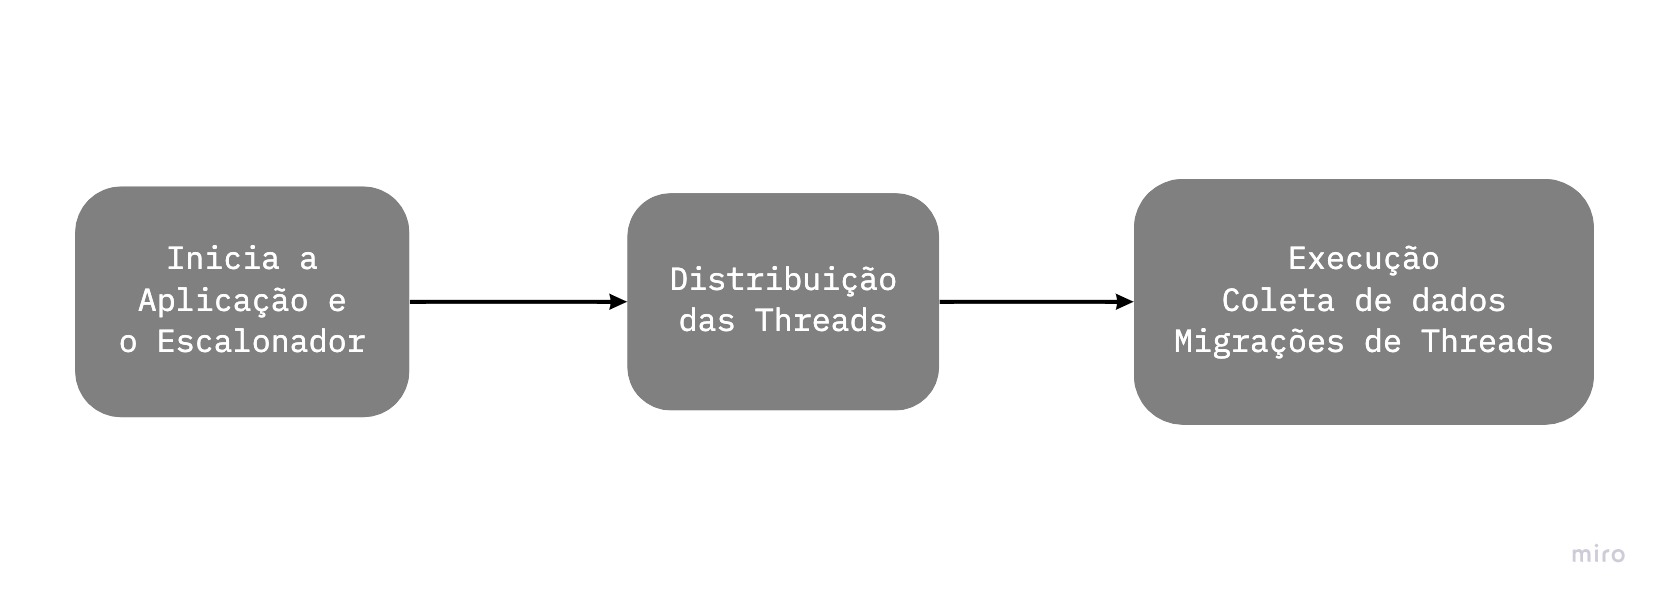
\includegraphics[scale=.25]{images/ltms_generic}
\caption{Fluxo de execução da LTMS} 
\label{ltms_generic}
\end{figure}

Ao inicializar uma aplicação o número de threads utilizados vai ser passado para o escalonador na chamada de sua biblioteca de threads, assim, o LTMS compara o número de threads da aplicação com a quantidade de cores da máquina, se o número de threads da aplicação for maior que o número de cores o LTMS cria uma fila para cada core, como visto na figura~\ref{queue_core}.

\begin{figure}[htbp]
  \centering
  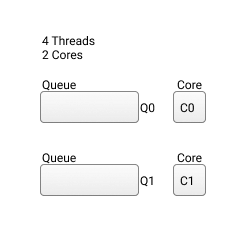
\includegraphics[scale=.8]{images/Queue_core.png}
  \caption{Criação das filas de execução com base nos cores}
\label{queue_core}
\end{figure}

Se a quantidade de threads da aplicação for menor que o número de cores disponível na arquitetura, o LTMS cria a mesma quantidade de filas que a quantidade de threads, fixando um core por fila e distribuindo uma thread por fila, como visto na figura~\ref{queue_thread}

\begin{figure}[htbp]
  \centering
  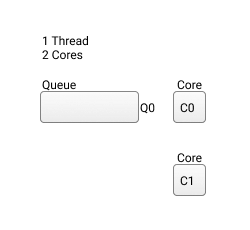
\includegraphics[scale=.8]{images/Queues_thread.png}
\caption{Criação das filas de execução com base nas threads} 
\label{queue_thread}
\end{figure}

% O escalonador se encarrega de distribuir inicialmente as threads entre as filas de execução com base em uma heuristica. O escalonador foi desenhado para que diferentes heurísticas possam ser desenvolvidas e acopladas a ele, permitindo testar diferentes formas de distribuição de threads. Neste trabalho foi desenvolvida uma heurística de distribuição de threads entre filas.

% \todo{
%   i: nota que tu ta misturando as coisas todas. tu tava falando de inicializacao, agora estas falando de coletas de dados e depois tu volta a falar da inicializacao. Acho melhor colocar aquela explicação do comentário F no inicio, depois quebras em seçoes especificas de inicializacao, tempo de execuçao, e migracao
% }
% Em tempo de execução o LTMS coleta as informações como, endereços de leitura e escrita mais utilizados, quais threads possuem a mesma afinidade de leitura e escrita, e a quantidade de commits e aborts existentes por thread.

% Caso ocorra um abort em uma transação, essas informações serão utilizadas para identificar qual fila a thread em execução tem maior afinidade caso sejá necessário executar uma migração.

% Para o LTMS decidir se deve migrar ou não uma thread de fila, foram desenvolvidas duas heurísticas que buscam minimizar o overhead do escalonador e aproveitar as características da arquitetura. Estas heurísticas de migrações serão detalhadas na subseção~\ref{migration_heuristic}.

Após a criação das filas de execução, conforme apresentado acima, as threads criadas na aplicação são distribuídas com base em uma heurística de distribuição, o escalonador foi desenhado para que diferentes heurísticas possam ser desenvolvidas e acopladas a ele, permitindo testar diferentes formas de distribuição de threads. Para este trabalho foram implementadas duas heurísticas de distribuição.

A primeira heurística implementada distribui uma thread por fila até a conclusão de todas threads disponíveis. A figura~\ref{queue_one} traz como exemplo 4 threads e 2 cores, neste caso serão criadas uma fila para cada core.

O escalonador executará a primeira fase de distribuição, colocando uma thread para cada fila existente. Após a primeira fase o escalonador verifica se ainda possui threads a serem distribuídas, caso hajam threads o LTMS repete a distribuição em uma segunda fase, até acabarem as threads.

Neste cenário a Fila intitulada Q0 fica com as threads t0 e t2, e a fila Q1 fica com as threads t1 e t3. Veja que o LTMS alocou a thread t0 em Q0 e depois alocou t1 em Q1, então voltou a execução para alocar t2 em Q0 e t3 em Q1.

\begin{figure}[htbp]
  \centering
  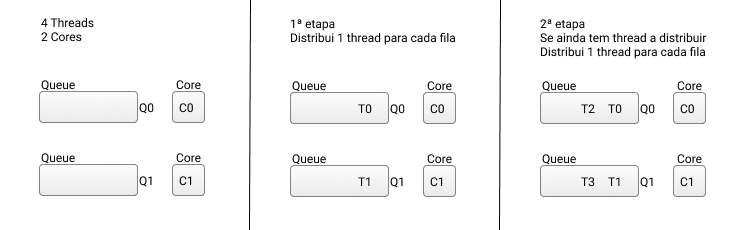
\includegraphics[scale=.6]{images/Queue_one.png}
\caption{Heurística um de distribuição de threads}
\label{queue_one}
\end{figure}

% \todo{
%   J: "A segunda heurística distribui duas threads por fila..."
% Mas isso é um exemplo específico correto? Ou não importa o número de threads e o número de cores ele sempre vai colocando de duas em duas?
% }

A segunda heurística distribui chunks de threads por fila, sendo o tamanho do chunk determinado pela razão entre a quantidade de threads e o quantidade de filas. No exemplo apresentado na figura~\ref{queue_two} temos o mesmo cenário de filas, cores e threads apresentados anteriormente.

% Na primeira fase de distribuição o escalonador aloca duas threads por fila, quando acabam as filas o escalonador verifica se há thread disponível para distribuição, se não há mais threads o LTMS encerra a distribuição. Caso haja apenas uma ultima thread para distribuir o escalonador aloca esta na fila em que parou a distribuição.

% Neste cenário o LTMS aloca na fila Q0 as threads t0 e t1, e na fila Q1 as threads t2 e t3.% Isto por que o escalonador alocou to e t1 em sequencia na fila Q0, para então alocar t2 e t3 na fila Q1.

\todo{arrumar}
\begin{figure}[htbp]
  \centering
  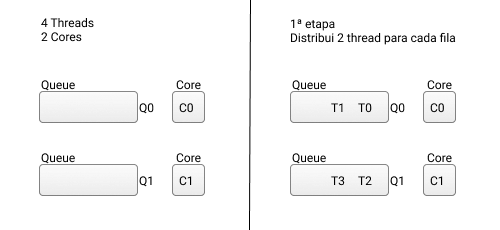
\includegraphics[scale=.8]{images/Queue_two.png}
\caption{Heurística dois de distribuição de threads}
\label{queue_two}
\end{figure}


\subsection{Coleta de dados em tempo de execução}
\label{coleta}

Durante a execução da aplicação o escalonador se encarrega de coletar dados de sua execução e da arquitetura utilizada para otimizar a redistribuição de threads entre as filas existentes caso ocorram aborts nas transações. Entre os dados coletados estão os acessos à memória, a quantidade de aborts e a quantidade de commits realizados pelos threads, também são coletados informações sobre os nodos NUMA existentes na arquitetura e os custos de latência existentes.

Os dados coletados sobre os acessos à memória fornecem insumos para duas matrizes, uma matriz de comunicação e uma matriz de endereços. Estas matrizes serão utilizadas nas heurísticas de migração para definir o grau de relação entre as filas de execução para reduzir os conflitos após uma migração de threads entre as filas.

A matriz de comunicação fornece insumos sobre a quantidade de vezes que duas threads acessam o mesmo endereçamento de memória. Os valores da matriz de comunicação se dão pelos somatórios dos acessos ao mesmo endereçamento de memória entre dois threads, sendo os identificadores dos threads as posições da matriz. Sendo assim se a thread com id 0 lê ou escreve 1000 vezes no mesmo endereço que a thread de id 1, o valor da matriz de comunicação na posição \emph{matrixComm[0][1]} será 1000.

Para evitar overhead a coleta de dados da matriz de comunicação ocorre por amostragem, neste trabalho utilizamos 1 a cada 100 acessos por thread para acionar o contador, esta mesma abordagem foi apresentada nos trabalhos~\cite{pasqualin2020online} e~\cite{pasqualin2020thread}. O LTMS permite que o valor da amostragem seja configurado, caso o desenvolvedor queira que todos os dados de acesso à memória sejam considerados.

A matriz de endereços por sua vez armazena a informação de quais endereços iguais foram acessados mais vezes pelas threads. Os valores da matriz de endereços são os endereçamentos de memória acessados mais vezes entre dois threads, e assim como na matriz de comunicação os identificadores dos threads são as posições da matriz. Assim, se a thread com id 0 e a thread de id 1 possuem mais acesse em comum com o endereço 0xbff6f36c, o valor da matriz de endereços na posição \emph{matrixAddress[0][1]} será 0xbff6f36c.

Para montar a matriz de endereços foi utilizado o mesmo sistema de amostragem apresentado anteriormente, no momento do armazenamento o endereço avaliado é armazenado em uma fila que é ordenada pela quantidade de acessos que o endereço recebeu, o endereço com maior número de acessos é armazenado na matriz de comunicação.

O LTMS também fica encarregado de coletar dados sobre o comportamento das transações. Durante sua execução uma thread pode ter n transações que geram aborts e commits, o escalonador mantem em cada thread um contador para os commits e um para os aborts. Esse contador mantem o histórico de commits e aborts de uma thread que será utilizado para identificar o índice de contenção da thread. 

\subsection{Migração de Threads}
\label{migracao}

O LTMS fornece um sistema de migração de threads entre as filas existentes, esse sistema entra em ação após a ocorrência de um abort e busca agrupar as threads conflitantes com intuito de serializadas para evitar conflitos futuros. O sistema de migração é dividido em duas etapas, a identificação da fila para a qual o thread será migrado e a heurística de migração que define se a migração ira acontecer.

A figura~\ref(migration) ilustra a função de migração denominada ~\emph(migrateThread), está função é executada após a ocorrência de um abort, a função~\emph{findBestQueue} identifica a fila para qual podemos efetuar a migração e a função~\emph{okToMigrate} utiliza uma heurística que determinar se devemos migrar a thread atual. Caso a thread deva ser migrada, a thread é adicionada a fila de execução para qual desejasse migra-la. Caso a thread não deva ser migrada, a função retorna para operação de abort e segue a execução utilizando o gerenciador de contenção.

\begin{figure}[htbp]
  \centering
  \begin{lstlisting}
    migrateThread(thread) {
      if (okToMigrate(thread))
        findBestQueue(thread).push();
    }
  \end{lstlisting}
  \caption{Função de migração}
  \label{migration}
\end{figure}

A etapa de identificação das threads conflitantes busca entender a aplicação e a arquitetura para definir para qual fila a thread que gerou o abort deve ser migrada, para isso a função~\emph{findBestQueue} recebe o identificador da thread atual e consulta na matriz de comunicação qual a thread em execução possui mais acessos em comum à memória, após identificar a thread a função retorna a fila na qual a thread pertence. Após identificar a fila com maior afinidade, o LTMS utiliza uma das heurísticas para decidir se migrará a thread ou não.

A etapa de heurística de migração avalia se a thread que gerou o abort está apta a ser migrada, o LTMS permite que diferentes heurísticas de migração sejam desenvolvidas e acopladas a ele.  Para este trabalho foram desenvolvidas duas heurísticas de migração, que avaliam os dados coletados para tomar a decisão de migrar a thread. Estas heurística foram denominadas \emph{threshold} e \emph{latency} e são apresentadas nas figuras~\ref{threshold} e~\ref{latency}.

A primeira heurística, denominada threshold, avalia o nível de contenção apresentado pela thread em tempo de execução, esse nível de contenção é medido pela razão entre os aborts e commits realizados pela thread, onde um resultado alto indica uma maior contenção ocasionada pelos aborts. Para realizar uma migração utilizando esta heurística o LTMS executa a função apresentada na figura\ref{threshold}.

A função \emph{thresholdHeuristic} apresentadas na figura~\ref{threshold} calcula o índice de contenção dado pela razão dos aborts e commits realizados pela thread e avalia se o índice de contenção é maior que um valor limiar. Se o índice de contenção for maior que o limiar a função permite a migração da thread, se o valor do índice de contenção ficar abaixo do limiar a thread não deve ser migrada.

O limiar denominado~\emph{threshold} é uma constante definida pelo desenvolvedor que indica o nível máximo de contenção aceito pela aplicação, um valor baixo para o limiar gera mais migrações que proporciona maior serialização do sistema reduzindo assim os aborts e aumentando tempo de execução, enquanto um limiar muito alto mantem o paralelismo mas aumenta o número de aborts.

\begin{figure}[htbp]
  \centering
  \begin{lstlisting}
    bool thresholdHeuristic(thread) {
      return thread.aborts/thread.commits >= threshold
    }
  \end{lstlisting}
  \caption{Heurística de migração threshold}
  \label{threshold}
\end{figure}

A segunda heurística de migração, denominada \emph{latency}, avalia a latência de acesso a memória entres os nodos da filas envolvidas na migração e o endereço de memória mais acessado pela thread. Para realizar uma migração utilizando esta heurística o LTMS executa a função denominada~\emph{latencyHeuristic} apresentada na figura\ref{latency}.

A função \emph{latencyHeuristic} busca na matriz de endereços qual o endereço de memória em comum é mais acessado pelas filas. A função também consulta quais os nodos NUMA a fila atual e a fila que está sendo avaliada pertencem. Com as informações sobre os nodos NUMA e o endereço de memória mais acessado, é avaliada as latências de acesso das duas filas para o endereço de memória, se a fila atual possui uma latência de acesso maior que a fila para a qual pretendemos migrar a thread o escalonador efetua a migração, caso a latência seja menor ou igual a thread mantem sua execução na fila atual.

Migrando a thread para uma fila com latência menor que a atual, o LTMS busca reduzir o número de aborts serializando parte da execução, e busca também aproveitar as características da arquitetura otimizando o acesso à memória dentro da região NUMA. A migração não ocorre se a latência da nova fila for maior para evitar futuros acessos entre diferentes nodos NUMA.

\begin{figure}[htbp]
  \centering
  \begin{lstlisting}
    bool latencyHeuristic(currentQueueId, nextQueueId) {
      address = getAddress(currentQueueId, nextQueueId)
      nodeNextQueue = getNodeNuma(nextQueueId.node)
      nodeCurrentQueue = getNodeNuma(currentQueueId.node)
      currentLatency = latency(nodeCurrentQueue, address)
      nextLatency = latency(nodeNextQueue, address)
      return currentLatency > nextLatency
    }
  \end{lstlisting}
  \caption{Heurística de migração latency}
\label{latency}
\end{figure}

\section{Conclusão}

Como visto na seção anterior o LTMS é um escalonador NUMA-Aware de tres etapas, a primeira se encarrega de inicializar a aplicação criando filas de execução e distribuindo as threads entre estas filas, a segunda etapa coleta dados sobre a arquitetura e a aplicação em tempo de execução para otimizar a aplicação por meio da serialização de threads conflitantes, a terceira etapa se encarrega de avaliar se uma thread que abortou deve ser serializada, a serialização ocorre por meio da migração da thread que realizou o abort para uma fila que possua as mesmas características de acesso à memória.

O escalonador permite a criação de diferentes heurísticas para avaliar seu comportamento de distribuição de threads na faze inicial e na migração de threads na ocorrência de aborts. Estas heurísticas podem ser criadas e acopladas ao LTMS para melhorar o fluxo de execução das aplicações e facilitar estudos futuros.

O LTMS é um escalonador reativo que realiza a faze de migração de threads a partir da ocorrência de um abort, como podemos ter mais de uma transação por thread os dados coletados para o sistema de migração são avaliados por threads, isto permite a comparação entre as características dos acessos à memória e o índice de contenção gerado por cada thread. Assim como o LTMS o Shirink~\cite{shirink2009} avalia as informações em tempo de execução com base nas threads, porem este não avalia as características de acesso à memória.

Algoritmos como LUTS~\cite{Nicacio2012} utilizam a migração para reduzir o índice de contenção, porem este algoritmo realiza a migração para uma única fila, serializando a aplicação sem considerar as características de acesso à memória. Outros algoritmos, como o ATS~\cite{ats2008} e o Shirink~\cite{shirink2009}, realizam a serialização sem efetuar uma migração, apenas controlando o número de threads ativos na aplicação o que reduz a contenção mas utiliza totalmente o recurso disponivel na arquitetura.

A tabela~\ref{tab:compare_ltms} apresenta uma comparação entre as principais características do LTMS e os escalonadores apresentados neste trabalho, a tabela busca entender as diferenças que o escalonador fornece para aplicações paralelas que utilizam STM.

\begin{table}[]
  \footnotesize
  \centering
  \caption{Comparativo entre os escalonadores aprensentados}
  \label{tab:compare_ltms}
  \begin{tabular}{l|l|l|l|l|l|l}
  \hline
  Escalonadores & LTMS & ATS & Shrink & LUTS & ProVIT & STMap \\ \hline %escalonadores
  Distribuição inicial de threads & Sim & Não & Não & Não & Não & Sim \\ 
  Coleta de dados por threads & Sim & Não & Sim & Sim & Sim & Sim \\
  Migração entre filas & Sim & Não & Não & Sim & Não & Não \\
  Avalia a arquitetura  & Sim & Não & Não & Não & Não & Sim \\
  Técnica de escalonamento & Reativo & Feedback & Predição & Mista & Mista & Predição \\ 
  \hline
  \end{tabular}
\end{table}

% \section{\textbf{Aplicação}}

% O LTMS é um escalonador de STM que inicializa sua execução junto com a aplicação e fornece todo suporte a memórias transacionais. A figura~\ref{LTMS1} apresenta o fluxo de execução de uma aplicação utilizando o LTMS.

% \begin{figure}[htbp]
%   \centering 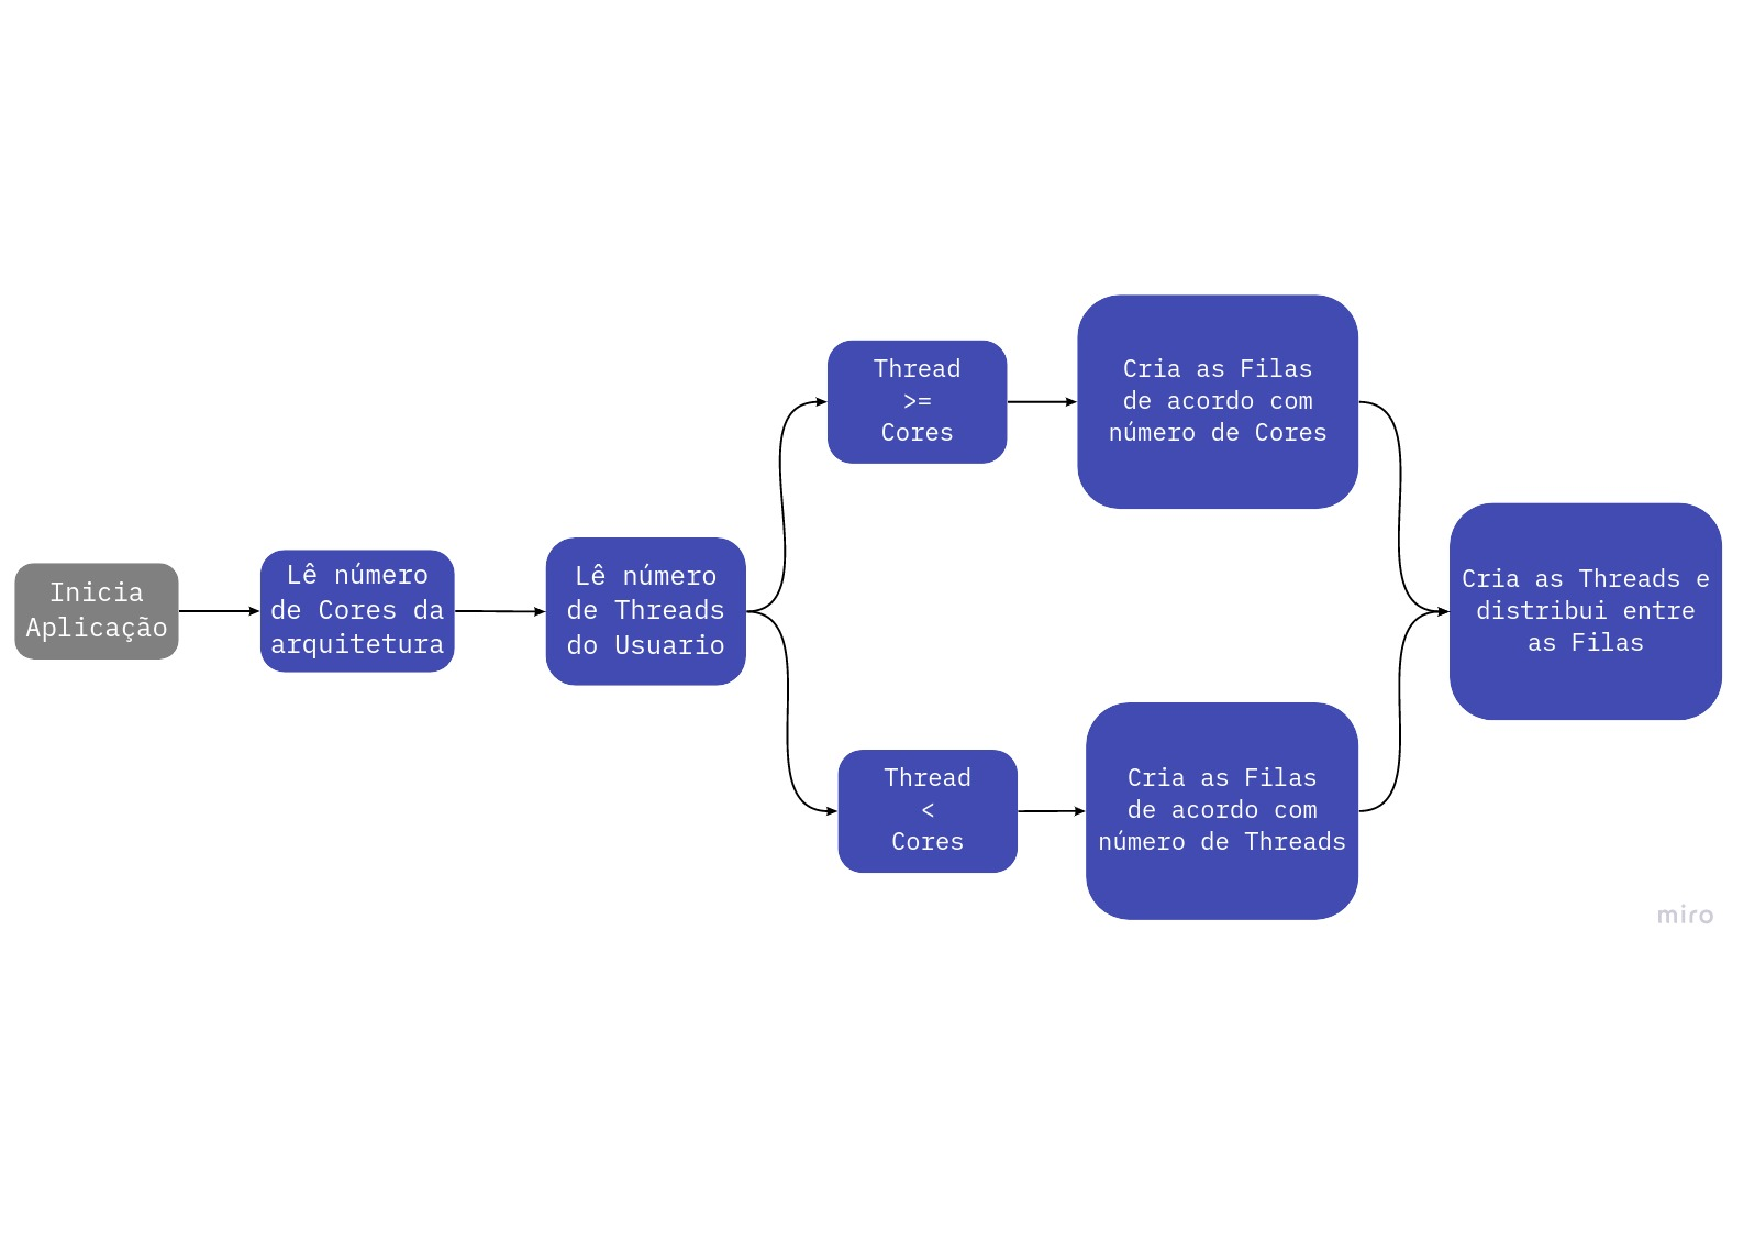
\includegraphics[scale=.5]{images/lstm1}
% \caption{Inicialização da LTMS} 
% \label{LTMS1}
% \end{figure}

% O escalonador foi desenvolvido em C++ para ser utilizado com a biblioteca de STM TinySTM. Para este trabalho foram utilizado os benchmarks do conjunto de benchmark STMAP.

% % Como visto na seção~\ref{section:stamp} o STAMP fornece uma biblioteca de thread chamada thread.h. O LTMS sobrepõem esta biblioteca fornecendo threads no padrão C++ 11 e uma serie de funções de escalonamento e mecanismos de distribuição de tarefas.

% A implementação do LTMS trás um conjunto de funções que utilizam recursos de threads do c++ para executar a aplicação junto com a biblioteca TinySTM. Estes ...

% % Para avaliar a arquitetura e entender o fluxo de execução foram utilizadas dentro do escalonador a biblioteca HwLoc e...

% ...

% \begin{figure}[htbp]
%   \centering 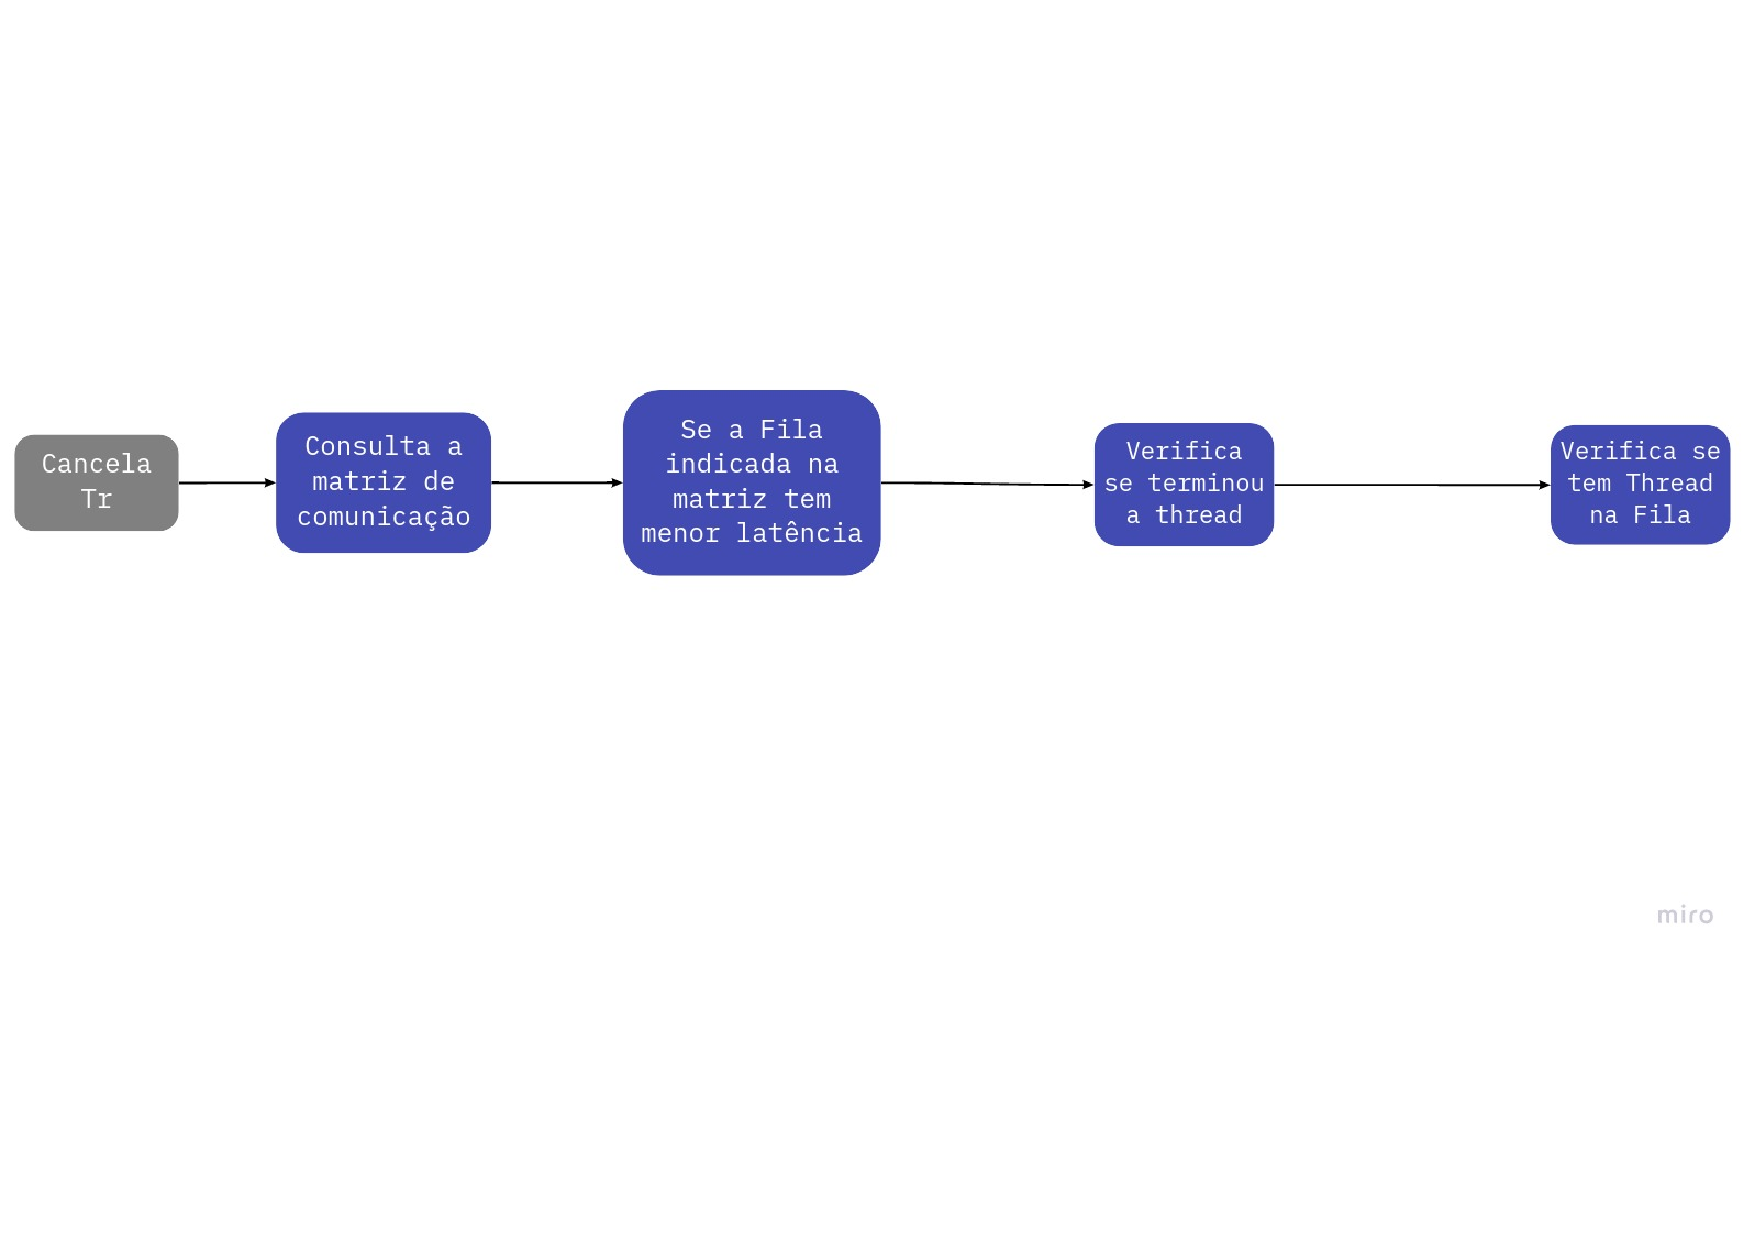
\includegraphics[scale=.5]{images/lstm2}
% \caption{Migração de threads na LTMS} 
% \label{LTMS2}
% \end{figure}

% ...

\chapter{Experimentos}
\label{chapter::experimentos}

Para este trabalho foi desenvolvida um escalonador de STM NUMA-Aware, entitulado LTMS, que funciona em três etapas. Para validação o escalonador LTMS foi desenvolvido em linguagem C, e aplicado à biblioteca de STM TinySTM em sua versão 1.0.5, e foram rodados esperimentos com o conjunto de benchmarks STMAP em sua versão 0.9.10.

Os testes foram rodados em uma máquina de arquitetura NUMA com processador Intel Xeon E5-4650 com 96 núcleos e 192 threads e 468 Gb de memória RAM, utilizando com sistema operacional Linux Debian kernel 4.19.0-8-amd64  e gcc 8.3.0.

Como comentado anteriormente o LTMS permite que heurísticas para distribuição de threads e heurísticas para migração de threads sejas desenvolvidas e acopladas a ele de maneira simples para que estudos possam ser realizados, neste trabalho foi desenvolvido duas heurísticas de distribuição e duas heurísticas de migração. Para obter os resultados do LTMS foram rodadas queatro baterias de testes com as seguintes configurações, LTMS com distribuição 1 e migração threshold, LTMS com distribuição 1 e migração latency, LTMS com distribuição 2 e migração threshold, e LTMS com distribuição 2 e migração latency. Para comparar o desenpenho do escalonador LTMS, foi executada uma bateria de teste com a TinySTM |todo{versão da tiny} sem modificações.

Cada bateria de teste consiste em 30 execuções de cada benchmark do conjunto STAMP, para os cenarios de 1, 2, 4, 8, 16, 32, 64, 128, 256, e 512 threads. A seção~\ref{resultados} mostra os resultados obtidos com os experimentos.

\section{Resultados}
\label{resultados}

\begin{figure}[!ht]
    % \centering
    \subfloat[Bayes]{
        \label{Bayes}
        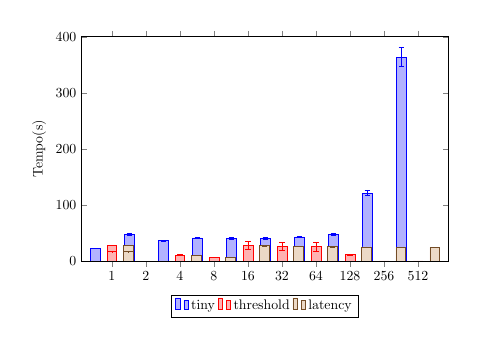
\begin{tikzpicture}[scale=0.5, baseline]
        \begin{axis}[
            width=0.9 \linewidth,
            height=0.6 \linewidth,
            %media de tempo intruder
            ybar=5pt,
            %enlargelimits=0.10,
            legend style={at={(0.5,-0.15)}, anchor=north, legend columns=-1},
            ylabel=Tempo(s),
            symbolic x coords={1, 2, 4, 8, 16, 32, 64, 128, 256, 512},
            xtick=data,
            ymin=0,
            ymax=400,
            bar width=7pt,
            % nodes near coords,
            nodes near coords align={vertical},
        ]
        \addplot+[error bars,y dir=both, y explicit] coordinates {
            (1,22.52)+-(1,0.13) (2,47.52)+-(2,1.02) (4,36.42)+-(4,0.57) (8,41.17)+-(8,1.22) (16,40.32)+-(16,1.21)
            (32,40.14)+-(32,2.42) (64,42.99)+-(64,1.48) (128,47.67)+-(128,2.37) (256,121.10)+-(256,4.24) (512,363.61)+-(512,17.08)}; %orininal
        \addplot+[error bars,y dir=both, y explicit] coordinates {
            (1,27.79)+-(1,0.15) (1,16.67)+-(2,0.18) (4,10.27)+-(4,0.86) (8,6.64)+-(8,0.34) (16,27.12)+-(16,7.19)
            (32,26.32)+-(32,7.19) (64,25.30)+-(64,7.72) (128,11.30)+-(128,0.42) (256,0.00)+-(256,0.0) (512,0.00)+-(512,0.0)}; %threshold
        \addplot+[error bars,y dir=both, y explicit] coordinates {
            (1,27.79)+-(1,0.13) (1,16.67)+-(2,0.13) (4,10.27)+-(4,0.13) (8,6.64)+-(8,0.13) (16,27.12)+-(16,0.13)
            (32,26.32)+-(32,0.13) (64,25.30)+-(64,0.13) (128,24.95)+-(128,0.13) (256,24.00)+-(256,0.13) (512,24.00)+-(512,0.13)}; %latency
        % \addplot coordinates {(1,405) (2,365) (4,338) (8,305) (16,263) (32,238) (64,225)}; %mainboard old
        \legend {tiny, threshold, latency}
        \end{axis}
        \end{tikzpicture}
    }
    \subfloat[Genome]{
        \label{Genome}
        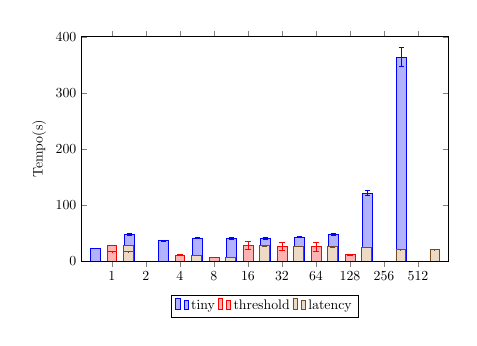
\begin{tikzpicture}[scale=0.5, baseline]
        \begin{axis}[
            width=0.9 \linewidth,
            height=0.6 \linewidth,
            %media de tempo intruder
            ybar=5pt,
            %enlargelimits=0.10,
            legend style={at={(0.5,-0.15)}, anchor=north, legend columns=-1},
            ylabel=Tempo(s),
            symbolic x coords={1, 2, 4, 8, 16, 32, 64, 128, 256, 512},
            xtick=data,
            ymin=0,
            ymax=400,
            bar width=7pt,
            % nodes near coords,
            nodes near coords align={vertical},
        ]
        \addplot+[error bars,y dir=both, y explicit] coordinates {
            (1,22.52)+-(1,0.13) (2,47.52)+-(2,1.02) (4,36.42)+-(4,0.57) (8,41.17)+-(8,1.22) (16,40.32)+-(16,1.21)
            (32,40.14)+-(32,2.42) (64,42.99)+-(64,1.48) (128,47.67)+-(128,2.37) (256,121.10)+-(256,4.24) (512,363.61)+-(512,17.08)}; %orininal
        \addplot+[error bars,y dir=both, y explicit] coordinates {
            (1,27.79)+-(1,0.15) (1,16.67)+-(2,0.18) (4,10.27)+-(4,0.86) (8,6.64)+-(8,0.34) (16,27.12)+-(16,7.19)
            (32,26.32)+-(32,7.19) (64,25.30)+-(64,7.72) (128,11.30)+-(128,0.42) (256,0.00)+-(256,0.0) (512,0.00)+-(512,0.0)}; %threshold
        \addplot+[error bars,y dir=both, y explicit] coordinates {
            (1,27.79)+-(1,0.13) (1,16.67)+-(2,0.13) (4,10.27)+-(4,0.13) (8,6.64)+-(8,0.13) (16,27.12)+-(16,0.13)
            (32,26.32)+-(32,0.13) (64,25.30)+-(64,0.13) (128,24.95)+-(128,0.13) (256,20.00)+-(256,0.13) (512,20.00)+-(512,0.13)}; %latency
        % \addplot coordinates {(1,405) (2,365) (4,338) (8,305) (16,263) (32,238) (64,225)}; %mainboard old
        \legend {tiny, threshold, latency}
        \end{axis}
        \end{tikzpicture}
    }
    
    \subfloat[Intruder]{
        \label{Intruder}
        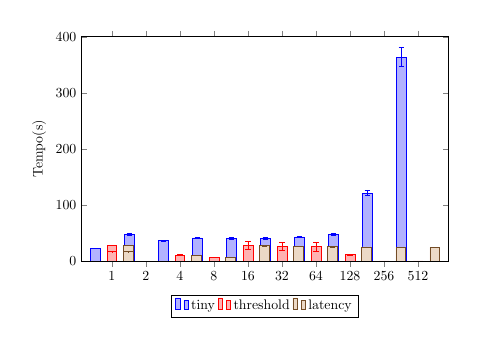
\begin{tikzpicture}[scale=0.5, baseline]
        \begin{axis}[
            width=0.9 \linewidth,
            height=0.6 \linewidth,
            %media de tempo intruder
            ybar=5pt,
            %enlargelimits=0.10,
            legend style={at={(0.5,-0.15)}, anchor=north, legend columns=-1},
            ylabel=Tempo(s),
            symbolic x coords={1, 2, 4, 8, 16, 32, 64, 128, 256, 512},
            xtick=data,
            ymin=0,
            ymax=400,
            bar width=7pt,
            % nodes near coords,
            nodes near coords align={vertical},
        ]
        \addplot+[error bars,y dir=both, y explicit] coordinates {
            (1,22.52)+-(1,0.13) (2,47.52)+-(2,1.02) (4,36.42)+-(4,0.57) (8,41.17)+-(8,1.22) (16,40.32)+-(16,1.21)
            (32,40.14)+-(32,2.42) (64,42.99)+-(64,1.48) (128,47.67)+-(128,2.37) (256,121.10)+-(256,4.24) (512,363.61)+-(512,17.08)}; %orininal
        \addplot+[error bars,y dir=both, y explicit] coordinates {
            (1,27.79)+-(1,0.15) (1,16.67)+-(2,0.18) (4,10.27)+-(4,0.86) (8,6.64)+-(8,0.34) (16,27.12)+-(16,7.19)
            (32,26.32)+-(32,7.19) (64,25.30)+-(64,7.72) (128,11.30)+-(128,0.42) (256,0.00)+-(256,0.0) (512,0.00)+-(512,0.0)}; %threshold
        \addplot+[error bars,y dir=both, y explicit] coordinates {
            (1,27.79)+-(1,0.13) (1,16.67)+-(2,0.13) (4,10.27)+-(4,0.13) (8,6.64)+-(8,0.13) (16,27.12)+-(16,0.13)
            (32,26.32)+-(32,0.13) (64,25.30)+-(64,0.13) (128,24.95)+-(128,0.13) (256,24.00)+-(256,0.13) (512,24.00)+-(512,0.13)}; %latency
        % \addplot coordinates {(1,405) (2,365) (4,338) (8,305) (16,263) (32,238) (64,225)}; %mainboard old
        \legend {tiny, threshold, latency}
        \end{axis}
        \end{tikzpicture}
    }
    \subfloat[Kmeans]{
        \label{Kmeans}
        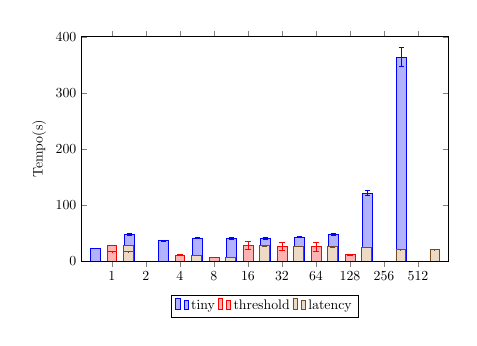
\begin{tikzpicture}[scale=0.5, baseline]
        \begin{axis}[
            width=0.9 \linewidth,
            height=0.6 \linewidth,
            %media de tempo intruder
            ybar=5pt,
            %enlargelimits=0.10,
            legend style={at={(0.5,-0.15)}, anchor=north, legend columns=-1},
            ylabel=Tempo(s),
            symbolic x coords={1, 2, 4, 8, 16, 32, 64, 128, 256, 512},
            xtick=data,
            ymin=0,
            ymax=400,
            bar width=7pt,
            % nodes near coords,
            nodes near coords align={vertical},
        ]
        \addplot+[error bars,y dir=both, y explicit] coordinates {
            (1,22.52)+-(1,0.13) (2,47.52)+-(2,1.02) (4,36.42)+-(4,0.57) (8,41.17)+-(8,1.22) (16,40.32)+-(16,1.21)
            (32,40.14)+-(32,2.42) (64,42.99)+-(64,1.48) (128,47.67)+-(128,2.37) (256,121.10)+-(256,4.24) (512,363.61)+-(512,17.08)}; %orininal
        \addplot+[error bars,y dir=both, y explicit] coordinates {
            (1,27.79)+-(1,0.15) (1,16.67)+-(2,0.18) (4,10.27)+-(4,0.86) (8,6.64)+-(8,0.34) (16,27.12)+-(16,7.19)
            (32,26.32)+-(32,7.19) (64,25.30)+-(64,7.72) (128,11.30)+-(128,0.42) (256,0.00)+-(256,0.0) (512,0.00)+-(512,0.0)}; %threshold
        \addplot+[error bars,y dir=both, y explicit] coordinates {
            (1,27.79)+-(1,0.13) (1,16.67)+-(2,0.13) (4,10.27)+-(4,0.13) (8,6.64)+-(8,0.13) (16,27.12)+-(16,0.13)
            (32,26.32)+-(32,0.13) (64,25.30)+-(64,0.13) (128,24.95)+-(128,0.13) (256,20.00)+-(256,0.13) (512,20.00)+-(512,0.13)}; %latency
        % \addplot coordinates {(1,405) (2,365) (4,338) (8,305) (16,263) (32,238) (64,225)}; %mainboard old
        \legend {tiny, threshold, latency}
        \end{axis}
        \end{tikzpicture}
    }

    \subfloat[Labyrinth]{
        \label{Labyrinth}
        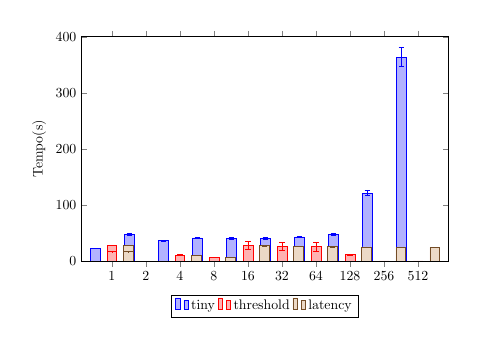
\begin{tikzpicture}[scale=0.5, baseline]
        \begin{axis}[
            width=0.9 \linewidth,
            height=0.6 \linewidth,
            %media de tempo intruder
            ybar=5pt,
            %enlargelimits=0.10,
            legend style={at={(0.5,-0.15)}, anchor=north, legend columns=-1},
            ylabel=Tempo(s),
            symbolic x coords={1, 2, 4, 8, 16, 32, 64, 128, 256, 512},
            xtick=data,
            ymin=0,
            ymax=400,
            bar width=7pt,
            % nodes near coords,
            nodes near coords align={vertical},
        ]
        \addplot+[error bars,y dir=both, y explicit] coordinates {
            (1,22.52)+-(1,0.13) (2,47.52)+-(2,1.02) (4,36.42)+-(4,0.57) (8,41.17)+-(8,1.22) (16,40.32)+-(16,1.21)
            (32,40.14)+-(32,2.42) (64,42.99)+-(64,1.48) (128,47.67)+-(128,2.37) (256,121.10)+-(256,4.24) (512,363.61)+-(512,17.08)}; %orininal
        \addplot+[error bars,y dir=both, y explicit] coordinates {
            (1,27.79)+-(1,0.15) (1,16.67)+-(2,0.18) (4,10.27)+-(4,0.86) (8,6.64)+-(8,0.34) (16,27.12)+-(16,7.19)
            (32,26.32)+-(32,7.19) (64,25.30)+-(64,7.72) (128,11.30)+-(128,0.42) (256,0.00)+-(256,0.0) (512,0.00)+-(512,0.0)}; %threshold
        \addplot+[error bars,y dir=both, y explicit] coordinates {
            (1,27.79)+-(1,0.13) (1,16.67)+-(2,0.13) (4,10.27)+-(4,0.13) (8,6.64)+-(8,0.13) (16,27.12)+-(16,0.13)
            (32,26.32)+-(32,0.13) (64,25.30)+-(64,0.13) (128,24.95)+-(128,0.13) (256,24.00)+-(256,0.13) (512,24.00)+-(512,0.13)}; %latency
        % \addplot coordinates {(1,405) (2,365) (4,338) (8,305) (16,263) (32,238) (64,225)}; %mainboard old
        \legend {tiny, threshold, latency}
        \end{axis}
        \end{tikzpicture}
    }
    \subfloat[SSCA2]{
        \label{SSCA2}
        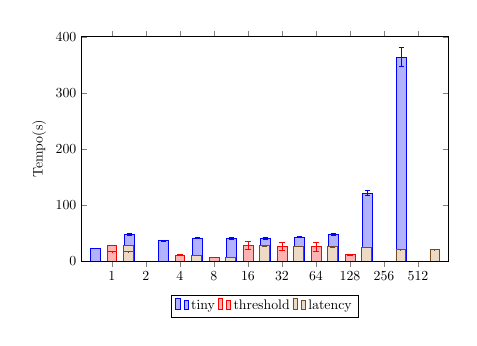
\begin{tikzpicture}[scale=0.5, baseline]
        \begin{axis}[
            width=0.9 \linewidth,
            height=0.6 \linewidth,
            %media de tempo intruder
            ybar=5pt,
            %enlargelimits=0.10,
            legend style={at={(0.5,-0.15)}, anchor=north, legend columns=-1},
            ylabel=Tempo(s),
            symbolic x coords={1, 2, 4, 8, 16, 32, 64, 128, 256, 512},
            xtick=data,
            ymin=0,
            ymax=400,
            bar width=7pt,
            % nodes near coords,
            nodes near coords align={vertical},
        ]
        \addplot+[error bars,y dir=both, y explicit] coordinates {
            (1,22.52)+-(1,0.13) (2,47.52)+-(2,1.02) (4,36.42)+-(4,0.57) (8,41.17)+-(8,1.22) (16,40.32)+-(16,1.21)
            (32,40.14)+-(32,2.42) (64,42.99)+-(64,1.48) (128,47.67)+-(128,2.37) (256,121.10)+-(256,4.24) (512,363.61)+-(512,17.08)}; %orininal
        \addplot+[error bars,y dir=both, y explicit] coordinates {
            (1,27.79)+-(1,0.15) (1,16.67)+-(2,0.18) (4,10.27)+-(4,0.86) (8,6.64)+-(8,0.34) (16,27.12)+-(16,7.19)
            (32,26.32)+-(32,7.19) (64,25.30)+-(64,7.72) (128,11.30)+-(128,0.42) (256,0.00)+-(256,0.0) (512,0.00)+-(512,0.0)}; %threshold
        \addplot+[error bars,y dir=both, y explicit] coordinates {
            (1,27.79)+-(1,0.13) (1,16.67)+-(2,0.13) (4,10.27)+-(4,0.13) (8,6.64)+-(8,0.13) (16,27.12)+-(16,0.13)
            (32,26.32)+-(32,0.13) (64,25.30)+-(64,0.13) (128,24.95)+-(128,0.13) (256,20.00)+-(256,0.13) (512,20.00)+-(512,0.13)}; %latency
        % \addplot coordinates {(1,405) (2,365) (4,338) (8,305) (16,263) (32,238) (64,225)}; %mainboard old
        \legend {tiny, threshold, latency}
        \end{axis}
        \end{tikzpicture}
    }

    \subfloat[Vacation]{
        \label{Vacation}
        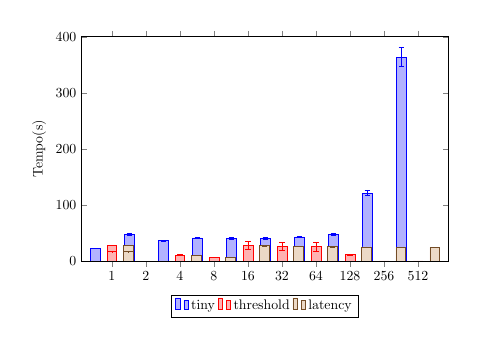
\begin{tikzpicture}[scale=0.5, baseline]
        \begin{axis}[
            width=0.9 \linewidth,
            height=0.6 \linewidth,
            %media de tempo intruder
            ybar=5pt,
            %enlargelimits=0.10,
            legend style={at={(0.5,-0.15)}, anchor=north, legend columns=-1},
            ylabel=Tempo(s),
            symbolic x coords={1, 2, 4, 8, 16, 32, 64, 128, 256, 512},
            xtick=data,
            ymin=0,
            ymax=400,
            bar width=7pt,
            % nodes near coords,
            nodes near coords align={vertical},
        ]
        \addplot+[error bars,y dir=both, y explicit] coordinates {
            (1,22.52)+-(1,0.13) (2,47.52)+-(2,1.02) (4,36.42)+-(4,0.57) (8,41.17)+-(8,1.22) (16,40.32)+-(16,1.21)
            (32,40.14)+-(32,2.42) (64,42.99)+-(64,1.48) (128,47.67)+-(128,2.37) (256,121.10)+-(256,4.24) (512,363.61)+-(512,17.08)}; %orininal
        \addplot+[error bars,y dir=both, y explicit] coordinates {
            (1,27.79)+-(1,0.15) (1,16.67)+-(2,0.18) (4,10.27)+-(4,0.86) (8,6.64)+-(8,0.34) (16,27.12)+-(16,7.19)
            (32,26.32)+-(32,7.19) (64,25.30)+-(64,7.72) (128,11.30)+-(128,0.42) (256,0.00)+-(256,0.0) (512,0.00)+-(512,0.0)}; %threshold
        \addplot+[error bars,y dir=both, y explicit] coordinates {
            (1,27.79)+-(1,0.13) (1,16.67)+-(2,0.13) (4,10.27)+-(4,0.13) (8,6.64)+-(8,0.13) (16,27.12)+-(16,0.13)
            (32,26.32)+-(32,0.13) (64,25.30)+-(64,0.13) (128,24.95)+-(128,0.13) (256,24.00)+-(256,0.13) (512,24.00)+-(512,0.13)}; %latency
        % \addplot coordinates {(1,405) (2,365) (4,338) (8,305) (16,263) (32,238) (64,225)}; %mainboard old
        \legend {tiny, threshold, latency}
        \end{axis}
        \end{tikzpicture}
    }
    \subfloat[Yada]{
        \label{Yada}
        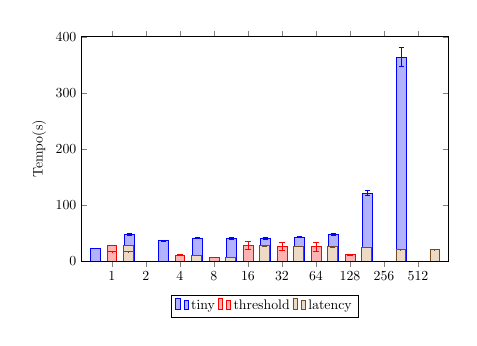
\begin{tikzpicture}[scale=0.5, baseline]
        \begin{axis}[
            width=0.9 \linewidth,
            height=0.6 \linewidth,
            %media de tempo intruder
            ybar=5pt,
            %enlargelimits=0.10,
            legend style={at={(0.5,-0.15)}, anchor=north, legend columns=-1},
            ylabel=Tempo(s),
            symbolic x coords={1, 2, 4, 8, 16, 32, 64, 128, 256, 512},
            xtick=data,
            ymin=0,
            ymax=400,
            bar width=7pt,
            % nodes near coords,
            nodes near coords align={vertical},
        ]
        \addplot+[error bars,y dir=both, y explicit] coordinates {
            (1,22.52)+-(1,0.13) (2,47.52)+-(2,1.02) (4,36.42)+-(4,0.57) (8,41.17)+-(8,1.22) (16,40.32)+-(16,1.21)
            (32,40.14)+-(32,2.42) (64,42.99)+-(64,1.48) (128,47.67)+-(128,2.37) (256,121.10)+-(256,4.24) (512,363.61)+-(512,17.08)}; %orininal
        \addplot+[error bars,y dir=both, y explicit] coordinates {
            (1,27.79)+-(1,0.15) (1,16.67)+-(2,0.18) (4,10.27)+-(4,0.86) (8,6.64)+-(8,0.34) (16,27.12)+-(16,7.19)
            (32,26.32)+-(32,7.19) (64,25.30)+-(64,7.72) (128,11.30)+-(128,0.42) (256,0.00)+-(256,0.0) (512,0.00)+-(512,0.0)}; %threshold
        \addplot+[error bars,y dir=both, y explicit] coordinates {
            (1,27.79)+-(1,0.13) (1,16.67)+-(2,0.13) (4,10.27)+-(4,0.13) (8,6.64)+-(8,0.13) (16,27.12)+-(16,0.13)
            (32,26.32)+-(32,0.13) (64,25.30)+-(64,0.13) (128,24.95)+-(128,0.13) (256,20.00)+-(256,0.13) (512,20.00)+-(512,0.13)}; %latency
        % \addplot coordinates {(1,405) (2,365) (4,338) (8,305) (16,263) (32,238) (64,225)}; %mainboard old
        \legend {tiny, threshold, latency}
        \end{axis}
        \end{tikzpicture}
    }
    
    \caption{Tempo de execução (s) em NUMA variando o número de \emph{threads}.}
    \label{temp}

\end{figure}

\begin{figure}[!ht]
    \centering
    \subfloat[Labyrinth]{
        \label{Labyrinth}
        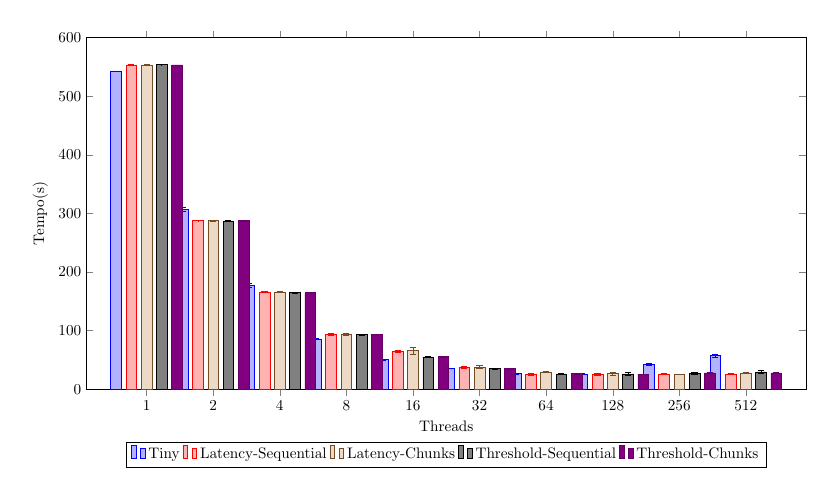
\begin{tikzpicture}[scale=0.55, baseline]
            \begin{axis}[
                width=1.5 \linewidth,
                height=0.8 \linewidth,
                %media de tempo intruder
                ybar=3pt,
                %enlargelimits=0.10,
                legend style={at={(0.5,-0.15)}, anchor=north, legend columns=-1},
                ylabel=Tempo(s),
            xlabel=Threads,
                symbolic x coords={1, 2, 4, 8, 16, 32, 64, 128, 256, 512},
                xtick=data,
                ymin=0,
                ymax=600,
                bar width=7pt,
                % nodes near coords,
                nodes near coords align={vertical},
            ]
            \addplot+[error bars,y dir=both, y explicit] coordinates {
                (1,543.12)+-(1,0.14) (2,307.12)+-(2,3.77) (4,177.18)+-(4,3.79) (8,86.06)+-(8,0.82) (16,50.63)+-(16,0.60) (32,35.89)+-(32,0.53) (64,26.45)+-(64,0.63) (128,25.83)+-(128,0.64) (256,41.98)+-(256,1.85) (512,57.32)+-(512,2.08) 
            };
            \addplot+[error bars,y dir=both, y explicit] coordinates {
                (1,553.57)+-(1,0.26) (2,287.70)+-(2,0.17) (4,165.86)+-(4,0.67) (8,94.13)+-(8,1.50) (16,65.04)+-(16,2.20) (32,37.22)+-(32,1.17) (64,25.60)+-(64,1.00) (128,25.49)+-(128,1.49) (256,26.10)+-(256,1.15) (512,25.80)+-(512,0.75)
            };
            \addplot+[error bars,y dir=both, y explicit] coordinates {
                (1,553.49)+-(1,0.21)(2,287.57)+-(2,0.25)(4,165.74)+-(4,0.99)(8,93.35)+-(8,1.29)(16,65.67)+-(16,6.11)(32,38.25)+-(32,1.76)(64,29.61)+-(64,0.77)(128,26.85)+-(128,2.24)(256,25.63)+-(256,0.42)(512,27.96)+-(512,1.35)
            };
            \addplot+[error bars,y dir=both, y explicit] coordinates {
                (1,553.89)+-(1,0.08) (2,287.30)+-(2,0.32) (4,164.88)+-(4,0.69) (8,93.33)+-(8,0.76) (16,55.06)+-(16,0.46) (32,35.27)+-(32,0.97) (64,26.35)+-(64,1.17) (128,26.33)+-(128,1.74) (256,26.96)+-(256,1.43) (512,29.70)+-(512,2.27) 
            };
            \addplot+[error bars,y dir=both, y explicit] coordinates {
                (1,553.38)+-(1,0.02) (2,287.58)+-(2,0.22) (4,164.99)+-(4,0.38) (8,93.83)+-(8,0.15) (16,55.92)+-(16,0.76) (32,35.17)+-(32,0.71) (64,26.79)+-(64,0.74) (128,25.67)+-(128,0.66) (256,27.99)+-(256,1.60) (512,28.01)+-(512,0.74)
            };
        \legend {Tiny, Latency-Sequential, Latency-Chunks, Threshold-Sequential, Threshold-Chunks}
        \end{axis}
        \end{tikzpicture}
    }

    \subfloat[Vacation]{
        \label{Vacation}
        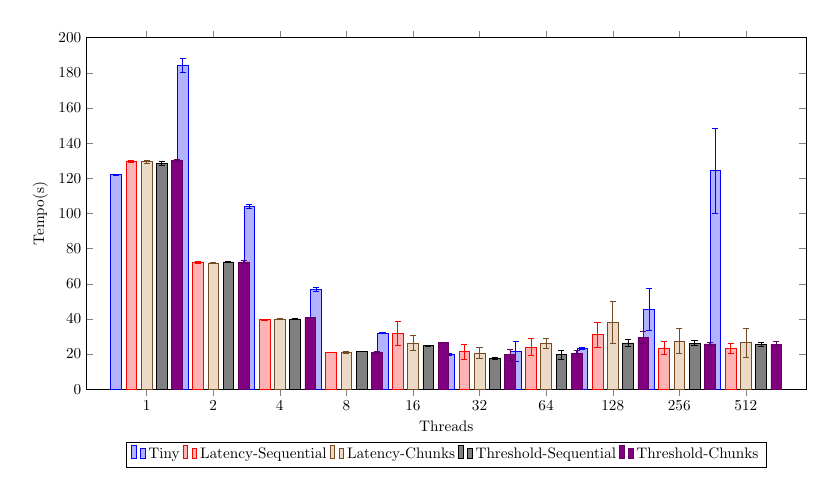
\begin{tikzpicture}[scale=0.55, baseline]
        \begin{axis}[
            width=1.5 \linewidth,
            height=0.8 \linewidth,
            %media de tempo intruder
            ybar=3pt,
            %enlargelimits=0.10,
            legend style={at={(0.5,-0.15)}, anchor=north, legend columns=-1},
            ylabel=Tempo(s),
            xlabel=Threads,
            symbolic x coords={1, 2, 4, 8, 16, 32, 64, 128, 256, 512},
            xtick=data,
            ymin=0,
            ymax=200,
            bar width=7pt,
            % nodes near coords,
            nodes near coords align={vertical},
        ]
        \addplot+[error bars,y dir=both, y explicit] coordinates {
            (1,122.19)+-(1,0.35) (2,184.47)+-(2,3.93) (4,103.92)+-(4,1.04) (8,56.80)+-(8,1.07) (16,31.99)+-(16,0.24) (32,19.69)+-(32,0.52) (64,21.68)+-(64,5.72) (128,23.22)+-(128,0.57) (256,45.58)+-(256,11.99) (512,124.45)+-(512,24.20) 
        };
        \addplot+[error bars,y dir=both, y explicit] coordinates {
            (1,129.87)+-(1,0.52) (2,72.20)+-(2,0.44) (4,39.59)+-(4,0.19) (8,21.14)+-(8,0.09) (16,31.78)+-(16,6.87) (32,21.39)+-(32,4.41) (64,24.02)+-(64,4.93) (128,31.01)+-(128,7.24) (256,23.53)+-(256,3.50) (512,23.21)+-(512,3.03)
        };
        \addplot+[error bars,y dir=both, y explicit] coordinates {
            (1,129.58)+-(1,0.88) (2,71.87)+-(2,0.48) (4,39.90)+-(4,0.39) (8,21.15)+-(8,0.64) (16,26.35)+-(16,4.18) (32,20.69)+-(32,3.15) (64,26.17)+-(64,3.04) (128,38.12)+-(128,12.03) (256,27.50)+-(256,7.32) (512,26.48)+-(512,8.21)
        };
        \addplot+[error bars,y dir=both, y explicit] coordinates {
            (1,128.56)+-(1,0.95) (2,72.45)+-(2,0.41) (4,40.00)+-(4,0.22) (8,21.55)+-(8,0.22) (16,24.76)+-(16,0.20) (32,17.51)+-(32,0.39) (64,19.62)+-(64,2.71) (128,26.34)+-(128,1.81) (256,26.30)+-(256,1.52) (512,25.59)+-(512,1.05) 
        };
        \addplot+[error bars,y dir=both, y explicit] coordinates {
            (1,130.29)+-(1,0.63) (2,72.49)+-(2,0.59) (4,40.83)+-(4,0.31) (8,21.11)+-(8,0.63) (16,26.56)+-(16,0.15) (32,19.76)+-(32,3.23) (64,20.45)+-(64,1.74) (128,29.49)+-(128,3.46) (256,25.76)+-(256,0.95) (512,25.70)+-(512,1.49)
        };
    \legend {Tiny, Latency-Sequential, Latency-Chunks, Threshold-Sequential, Threshold-Chunks}
        \end{axis}
        \end{tikzpicture}
    }

    \subfloat[Yada]{
        \label{Yada}
        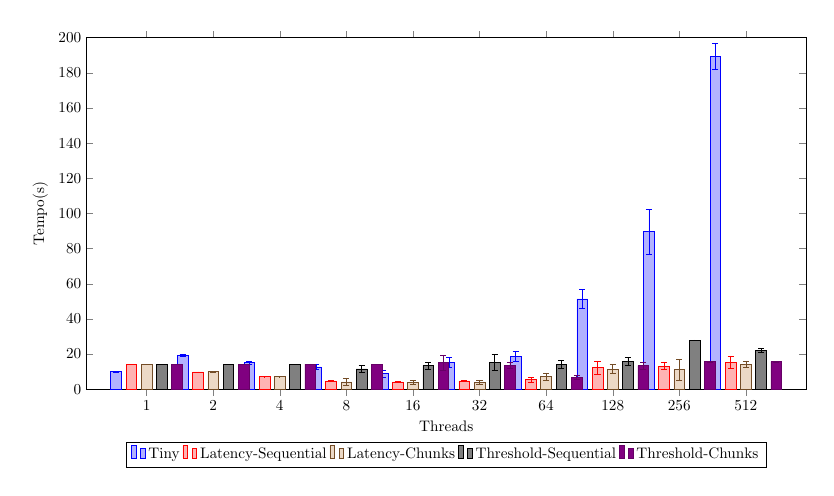
\begin{tikzpicture}[scale=0.55, baseline]
        \begin{axis}[
            width=1.5 \linewidth,
            height=0.8 \linewidth,
            %media de tempo intruder
            ybar=3pt,
            %enlargelimits=0.10,
            legend style={at={(0.5,-0.15)}, anchor=north, legend columns=-1},
            ylabel=Tempo(s),
            xlabel=Threads,
            symbolic x coords={1, 2, 4, 8, 16, 32, 64, 128, 256, 512},
            xtick=data,
            ymin=0,
            ymax=200,
            bar width=7pt,
            % nodes near coords,
            nodes near coords align={vertical},
        ]
        \addplot+[error bars,y dir=both, y explicit] coordinates {
            (1,9.95)+-(1,0.09) (2,19.42)+-(2,0.50) (4,15.05)+-(4,1.07) (8,12.75)+-(8,1.30) (16,8.85)+-(16,1.90) (32,15.25)+-(32,2.69) (64,18.85)+-(64,2.74) (128,51.34)+-(128,5.50) (256,89.66)+-(256,12.90) (512,189.43)+-(512,7.63) 
        };
        \addplot+[error bars,y dir=both, y explicit] coordinates {
            (1,14.09)+-(1,0.09) (2,9.88)+-(2,0.04) (4,7.22)+-(4,0.04) (8,4.78)+-(8,0.29) (16,4.19)+-(16,0.35) (32,4.74)+-(32,0.50) (64,5.38)+-(64,1.21) (128,12.38)+-(128,3.72) (256,13.14)+-(256,2.01) (512,15.43)+-(512,3.54)
        };
        \addplot+[error bars,y dir=both, y explicit] coordinates {
            (1,14.31)+-(1,0.16) (2,9.98)+-(2,0.07) (4,7.23)+-(4,0.11) (8,4.19)+-(8,1.93) (16,3.85)+-(16,0.97) (32,3.96)+-(32,1.37) (64,7.11)+-(64,1.83) (128,11.47)+-(128,2.48) (256,11.12)+-(256,5.94) (512,14.17)+-(512,1.47)
        };
        \addplot+[error bars,y dir=both, y explicit] coordinates {
            (1,14.17)+-(1,0.05) (2,14.17)+-(2,0.11) (4,14.20)+-(4,0.08) (8,11.61)+-(8,2.13) (16,13.53)+-(16,1.93) (32,15.15)+-(32,4.48) (64,14.19)+-(64,2.00) (128,15.69)+-(128,2.21) (256,27.92)+-(256,0.20) (512,22.18)+-(512,1.28) 
        };
        \addplot+[error bars,y dir=both, y explicit] coordinates {
            (1,14.35)+-(1,0.05) (2,14.29)+-(2,0.04) (4,14.31)+-(4,0.08) (8,14.31)+-(8,0.05) (16,15.07)+-(16,4.06) (32,13.64)+-(32,1.83) (64,6.83)+-(64,1.09) (128,13.37)+-(128,2.19) (256,15.65)+-(256,0.16) (512,15.73)+-(512,0.14)
        };
        \legend {Tiny, Latency-Sequential, Latency-Chunks, Threshold-Sequential, Threshold-Chunks}
        \end{axis}
        \end{tikzpicture}
    }
    
    \caption{Tempo de execução (s) em NUMA variando o número de \emph{threads}.}
    \label{temp2}

\end{figure}


\begin{figure}[!ht]
    \centering
    \subfloat[Bayes]{
        \label{Bayes}
        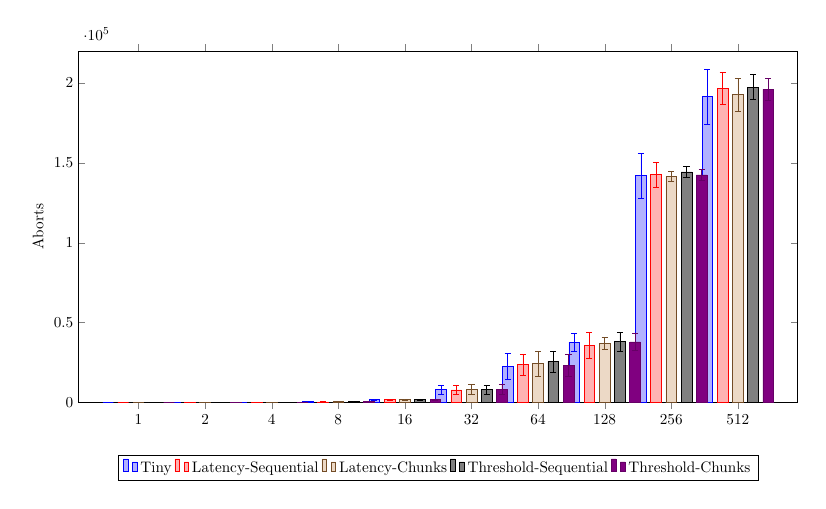
\begin{tikzpicture}[scale=0.55, baseline]
        \begin{axis}[
            width=1.5 \linewidth,
            height=0.8 \linewidth,
            %media de tempo intruder
            ybar=3pt,
            %enlargelimits=0.10,
            legend style={at={(0.5,-0.15)}, anchor=north, legend columns=-1},
            ylabel=Aborts,
            symbolic x coords={1, 2, 4, 8, 16, 32, 64, 128, 256, 512},
            xtick=data,
            ymin=0,
            ymax=220000,
            bar width=7pt,
            % nodes near coords,
            nodes near coords align={vertical},
        ]
        \addplot+[error bars,y dir=both, y explicit] coordinates {
            (1,0.0)+-(1,0.0) (2,35.0)+-(2,6.72) (4,111.0)+-(4,25.13) (8,470.6)+-(8,101.19) (16,1858.6)+-(16,343.71) (32,8018.2)+-(32,3060.82) (64,22527.4)+-(64,8121.85) (128,37743.2)+-(128,5565.49) (256,141872.2)+-(256,13892.27) (512,191436.8)+-(512,17258.39)
        };
        \addplot+[error bars,y dir=both, y explicit] coordinates {
            (1,0.0)+-(1,0.0) (2,23.0)+-(2,6.23) (4,126.0)+-(4,32.76) (8,440.6)+-(8,99.82) (16,1800.2)+-(16,399.13) (32,7936.18)+-(32,2798.23) (64,23847.2)+-(64,6522.42) (128,35938.5)+-(128,8262.18) (256,142628.8)+-(256,7947.57) (512,196582.3)+-(512,9788.9)
        };
        \addplot+[error bars,y dir=both, y explicit] coordinates {
            (1,0.0)+-(1,0.0) (2,37.0)+-(2,7.7) (4,131.4)+-(4,34.43) (8,455.22)+-(8,97.63) (16,1798.25)+-(16,285.341) (32,8134.4)+-(32,3281.67) (64,24227.4)+-(64,7812.5) (128,36972.9)+-(128,3907.18) (256,141539.2)+-(256,3362.2) (512,192748.4)+-(512,10239.43)
        };
        \addplot+[error bars,y dir=both, y explicit] coordinates {
            (1,0.0)+-(1,0.0) (2,29.0)+-(2,3.55) (4,127.0)+-(4,22.63) (8,487.9)+-(8,111.47) (16,1929.2)+-(16,317.1) (32,8063.21)+-(32,2840.32) (64,25728.67)+-(64,6565.8) (128,38082.222)+-(128,5736.93) (256,144284.24)+-(256,3475.15) (512,197398.8)+-(512,7834.42)
        };
        \addplot+[error bars,y dir=both, y explicit] coordinates {
            (1,0.0)+-(1,0.0) (2,35.0)+-(2,6.72) (4,114.94)+-(4,29.3) (8,494.33)+-(8,137.9) (16,1898.36)+-(16,364.82) (32,8082.64)+-(32,3019.92) (64,23189.6)+-(64,6989.99) (128,37964.7)+-(128,5387.7) (256,142367.33)+-(256,3478.75) (512,195893.8)+-(512,6746.09)
        };
        \legend {Tiny, Latency-Sequential, Latency-Chunks, Threshold-Sequential, Threshold-Chunks}
        \end{axis}
        \end{tikzpicture}
    }
    
    \subfloat[Intruder]{
        \label{Intruder}
        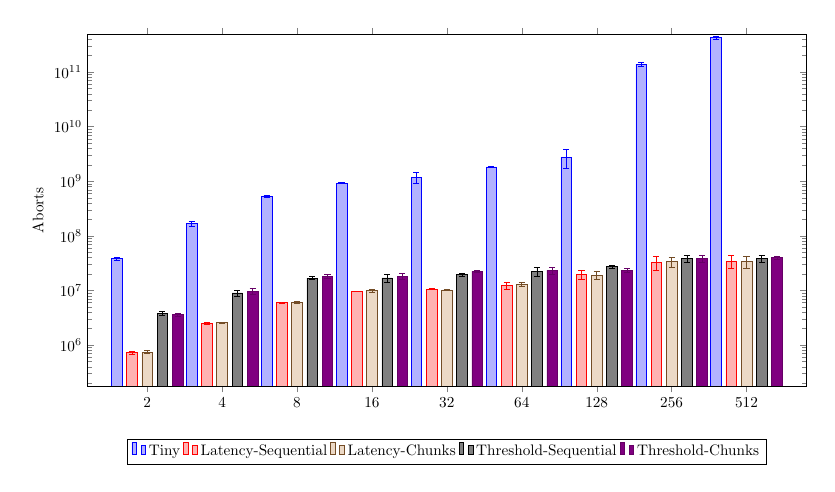
\begin{tikzpicture}[scale=0.55, baseline]
        \begin{axis}[
            ymode=log,
            width=1.5 \linewidth,
            height=0.8 \linewidth,
            %media de tempo intruder
            ybar=3pt,
            %enlargelimits=0.10,
            legend style={at={(0.5,-0.15)}, anchor=north, legend columns=-1},
            ylabel=Aborts,
            symbolic x coords={1, 2, 4, 8, 16, 32, 64, 128, 256, 512},
            xtick=data,
            ymin=0,
            ymax=490000000000,
            bar width=7pt,
            % nodes near coords,
            nodes near coords align={vertical},
        ]
        \addplot+[error bars,y dir=both, y explicit] coordinates {
            (1,0.0)+-(1,0.0) (2,38000260.8)+-(2,2949711.678076852) (4,166325696.4)+-(4,18557044.648063533) (8,529197870.6)+-(8,22132676.255908735) (16,924927047.6)+-(16,24358107.18760883) (32,1183579117.4)+-(32,270222169.9344623) (64,1831169740.8)+-(64,62890886.257802844) (128,2763435636.6)+-(128,1003746150.3805901) (256,138779112147.6)+-(256,10430244205.851603) (512,431443096033.6)+-(512,28705521954.994297) 
        };
        \addplot+[error bars,y dir=both, y explicit] coordinates {
            (1,0.0)+-(1,0.0) (2,724967.4)+-(2,38086.07014959669) (4,2505616.2)+-(4,79429.60770745378) (8,6012716.4)+-(8,169677.49348290125) (16,9639253.0)+-(16,142573.7883104745) (32,10568731.0)+-(32,292443.9680909832) (64,12171771.4)+-(64,1784435.4526392485) (128,19342142.8)+-(128,3669581.5184994815) (256,32980054.25)+-(256,9356623.644361822) (512,34119006.5)+-(512,8983159.5)
        };
        \addplot+[error bars,y dir=both, y explicit] coordinates {
             (1,0.0)+-(1,0.0) (2,745630.2)+-(2,40338.85590792084) (4,2559770.6)+-(4,81679.883166175) (8,6127472.777777778)+-(8,267489.386445634) (16,9889825.3)+-(16,755124.9867329315) (32,10236117.3)+-(32,288410.38292407227) (64,13078693.1)+-(64,982436.3361754746) (128,19063545.666666668)+-(128,2925827.5185046173) (256,33704832.6)+-(256,6772680.448815952) (512,34183921.0)+-(512,8274893.22) 
        };
        \addplot+[error bars,y dir=both, y explicit] coordinates {
            (1,0.0)+-(1,0.0) (2,3808172.2)+-(2,327085.8815720422) (4,9023407.8)+-(4,1123234.4180183227) (8,16872564.2)+-(8,1114383.5354166715) (16,17004377.2)+-(16,2666034.739783216) (32,19648666.0)+-(32,1287522.1930899676) (64,22307089.8)+-(64,4029768.617032169) (128,27162139.0)+-(128,1504557.0) (256,38132893.15)+-(256,4958389.304) (512,37984673.0)+-(512,5282793.33)
        };
        \addplot+[error bars,y dir=both, y explicit] coordinates {
            (1,0.0)+-(1,0.0) (2,3578932.78)+-(2,176854.86) (4,9738434.34)+-(4,1124342.85) (8,17928374.6)+-(8,1573847.9) (16,18301736.6)+-(16,2468736.987185277) (32,22436982.0)+-(32,1106602.0) (64,23420167.2)+-(64,3281430.727250502) (128,23366253.0)+-(128,1919489.0) (256,38736187.88)+-(256,5748878.34) (512,39763372.723)+-(512,3174827.12)
        };
        \legend {Tiny, Latency-Sequential, Latency-Chunks, Threshold-Sequential, Threshold-Chunks}
        \end{axis}
        \end{tikzpicture}
    }

    \subfloat[Kmeans]{
        \label{Kmeans}
        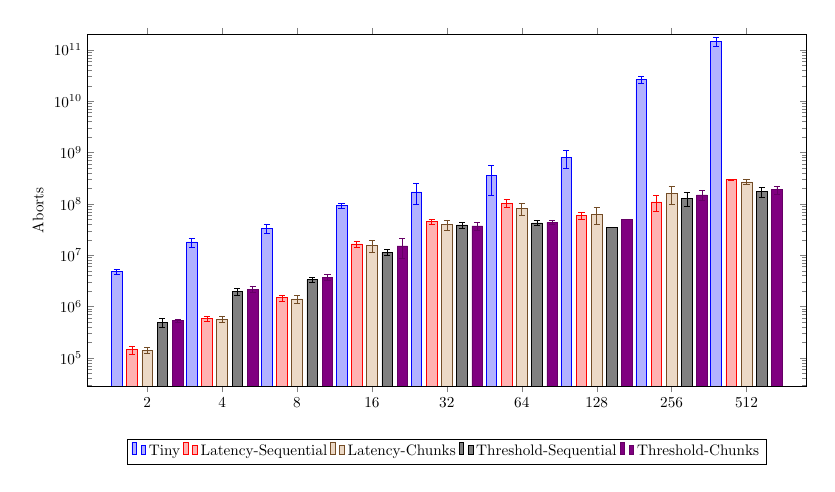
\begin{tikzpicture}[scale=0.55, baseline]
        \begin{axis}[
            ymode=log,
            width=1.5 \linewidth,
            height=0.8 \linewidth,
            %media de tempo intruder
            ybar=3pt,
            %enlargelimits=0.10,
            legend style={at={(0.5,-0.15)}, anchor=north, legend columns=-1},
            ylabel=Aborts,
            symbolic x coords={1, 2, 4, 8, 16, 32, 64, 128, 256, 512},
            xtick=data,
            ymin=0,
            ymax=200000000000,
            bar width=7pt,
            % nodes near coords,
            nodes near coords align={vertical},
        ]
        \addplot+[error bars,y dir=both, y explicit] coordinates {
            (1,0.0)+-(1,0.0) (2,4797421.2)+-(2,479774.7418784778) (4,18101846.8)+-(4,3591708.3539415835) (8,33182746.2)+-(8,6732288.556793311) (16,93057923.8)+-(16,9863144.322012922) (32,171442797.6)+-(32,74829388.10384364) (64,359745893.2)+-(64,213043475.04545623) (128,807753260.2)+-(128,310719932.9857997) (256,26569175006.4)+-(256,4470117158.120106) (512,146296330743.6)+-(512,26886172215.929005) 
        };
        \addplot+[error bars,y dir=both, y explicit] coordinates {
            (1,0.0)+-(1,0.0) (2,144295.6)+-(2,24864.282793597726) (4,579330.6)+-(4,68221.2484981036) (8,1486520.2)+-(8,200173.524986098) (16,16580311.4)+-(16,2227873.6890443857) (32,45063610.6)+-(32,5053643.0020858655) (64,103498202.6)+-(64,18052939.09375) (128,59441333.6)+-(128,8917614.717479235) (256,109146323.8)+-(256,36880499.382352196) (512,294773353.4)+-(512,3281309.7536428105)
        };
        \addplot+[error bars,y dir=both, y explicit] coordinates {
             (1,0.0)+-(1,0.0) (2,141609.1)+-(2,19957.913370139675) (4,570320.1)+-(4,69142.6626511447) (8,1412101.5)+-(8,239771.55806068826) (16,15454899.8)+-(16,3814349.1856658272) (32,39591108.222222224)+-(32,9286948.71968007) (64,81659510.1)+-(64,21584431.489666473) (128,62701912.9)+-(128,22625798.149042867) (256,157892521.1)+-(256,60541141.358650364) (512,267641468.75)+-(512,32356420.707834) 
        };
        \addplot+[error bars,y dir=both, y explicit] coordinates {
            (1,0.0)+-(1,0.0) (2,489474.6)+-(2,95557.56667391652) (4,1982817.6)+-(4,324496.7328282983) (8,3338695.4)+-(8,339537.1836017964) (16,11407592.4)+-(16,1467579.9615602007) (32,38923440.666666664)+-(32,5311247.22872386) (64,42424191.0)+-(64,4907763.0) (128,34826711.0)+-(128,578473.0) (256,128783746.63)+-(256,37482783.86) (512,173847878.28)+-(512,37384778.0)
        };
        \addplot+[error bars,y dir=both, y explicit] coordinates {
            (1,0.0)+-(1,0.0) (2,528574.7)+-(2,29384.0) (4,2157923.0)+-(4,283746.0) (8,3736425.62)+-(8,429388.0) (16,15208687.0)+-(16,6397145.233711557) (32,37279545.0)+-(32,6425946.0) (64,43456253.0)+-(64,3849829.0) (128,49875516.0)+-(128,675193.0) (256,148983127.32)+-(256,31827833.0) (512,187678278.0)+-(512,32738943.73)
        };
        \legend {Tiny, Latency-Sequential, Latency-Chunks, Threshold-Sequential, Threshold-Chunks}
        \end{axis}
        \end{tikzpicture}
    }
    
    \caption{Aborts em NUMA variando o número de \emph{threads}.}
    \label{abort}

\end{figure}


\begin{figure}[!ht]
    \centering
    \subfloat[Labyrinth]{
        \label{abortLabyrinth}
        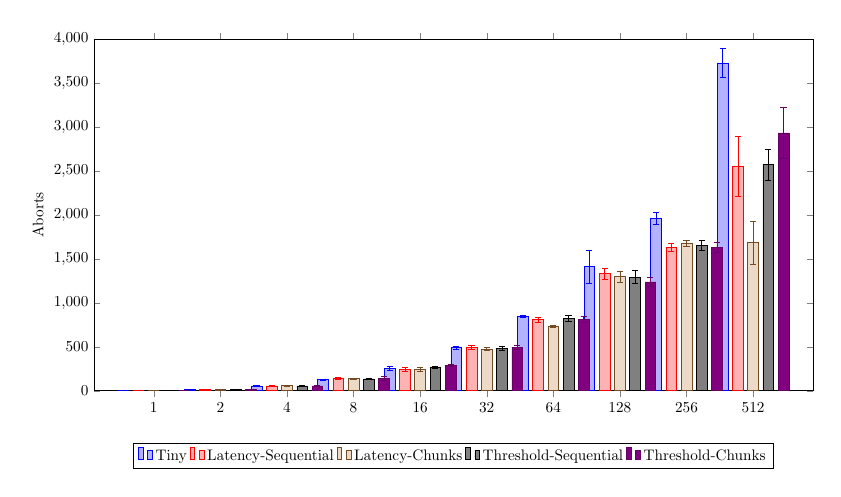
\begin{tikzpicture}[scale=0.55, baseline]
        \begin{axis}[
            width=1.5 \linewidth,
            height=0.8 \linewidth,
            %media de tempo intruder
            ybar=3pt,
            %enlargelimits=0.10,
            legend style={at={(0.5,-0.15)}, anchor=north, legend columns=-1},
            ylabel=Aborts,
            symbolic x coords={1, 2, 4, 8, 16, 32, 64, 128, 256, 512},
            xtick=data,
            ymin=0,
            ymax=4000,
            bar width=7pt,
            % nodes near coords,
            nodes near coords align={vertical},
        ]
        \addplot+[error bars,y dir=both, y explicit] coordinates {
            (1,0.0)+-(1,0.0) (2,12.2)+-(2,2.63) (4,53.2)+-(4,5.94) (8,127.2)+-(8,6.14) (16,258.0)+-(16,24.04) (32,490.2)+-(32,16.41) (64,847.0)+-(64,12.39) (128,1413.4)+-(128,186.85) (256,1959.6)+-(256,67.08) (512,3727.2)+-(512,167.11) 
        };
        \addplot+[error bars,y dir=both, y explicit] coordinates {
            (1,0.0)+-(1,0.0) (2,11.4)+-(2,0.48) (4,56.0)+-(4,4.09) (8,142.0)+-(8,12.85) (16,245.8)+-(16,19.87) (32,491.2)+-(32,25.11) (64,811.8)+-(64,28.18) (128,1334.2)+-(128,63.09) (256,1633.4)+-(256,41.57) (512,2556.6)+-(512,340.72)
        };
        \addplot+[error bars,y dir=both, y explicit] coordinates {
             (1,0.0)+-(1,0.0) (2,12.2)+-(2,1.46) (4,56.4)+-(4,3.61) (8,136.4)+-(8,10.30) (16,245.4)+-(16,19.39) (32,473.2)+-(32,16.47) (64,734.8)+-(64,11.12) (128,1298.4)+-(128,60.09) (256,1677.2)+-(256,35.19) (512,1686.8)+-(512,244.04)
        };
        \addplot+[error bars,y dir=both, y explicit] coordinates {
            (1,0.0)+-(1,0.0) (2,11.8)+-(2,0.97) (4,54.8)+-(4,2.78) (8,134.8)+-(8,4.39) (16,271.2)+-(16,11.35) (32,482.8)+-(32,22.57) (64,822.0)+-(64,36.78) (128,1291.2)+-(128,74.59) (256,1657.8)+-(256,58.13) (512,2571.6)+-(512,174.36)
        };
        \addplot+[error bars,y dir=both, y explicit] coordinates {
            (1,0.0)+-(1,0.0) (2,11.0)+-(2,1.2) (4,55.72)+-(4,10.82) (8,143.2)+-(8,25.75) (16,286.0)+-(16,10.86) (32,496.6)+-(32,19.73) (64,812.0)+-(64,38.57) (128,1238.6)+-(128,53.69) (256,1629.6)+-(256,55.64) (512,2933.4)+-(512,289.46)
        };
        \legend {Tiny, Latency-Sequential, Latency-Chunks, Threshold-Sequential, Threshold-Chunks}
        \end{axis}
        \end{tikzpicture}
    }
    
    \subfloat[Vacation]{
        \label{abortVacation}
        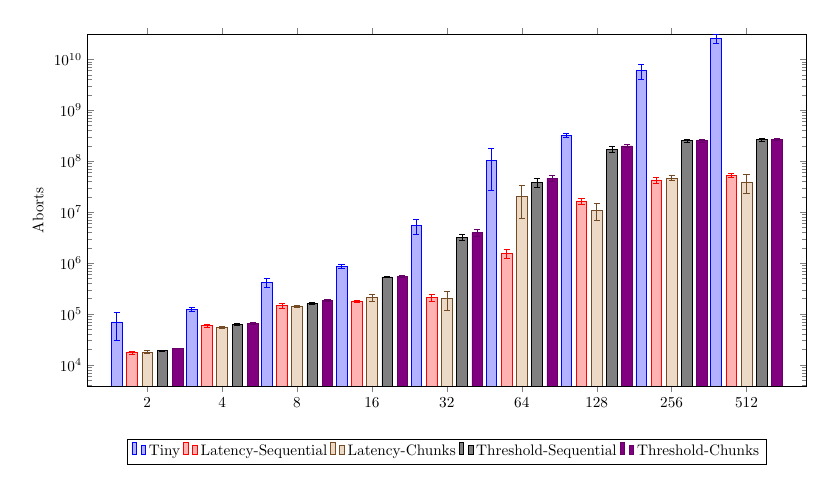
\begin{tikzpicture}[scale=0.55, baseline]
        \begin{axis}[
            ymode=log,
            width=1.5 \linewidth,
            height=0.8 \linewidth,
            %media de tempo intruder
            ybar=3pt,
            %enlargelimits=0.10,
            legend style={at={(0.5,-0.15)}, anchor=north, legend columns=-1},
            ylabel=Aborts,
            symbolic x coords={1, 2, 4, 8, 16, 32, 64, 128, 256, 512},
            xtick=data,
            ymin=0,
            ymax=31000000000,
            bar width=7pt,
            % nodes near coords,
            nodes near coords align={vertical},
        ]
        \addplot+[error bars,y dir=both, y explicit] coordinates {
            (1,0.0)+-(1,0.0) (2,69940.4)+-(2,38859.442881235445) (4,123224.4)+-(4,10230.047558051723) (8,421702.0)+-(8,83144.47432752221) (16,858817.0)+-(16,70319.27963794851) (32,5482927.6)+-(32,1822574.306164838) (64,102125071.2)+-(64,75531726.60526115) (128,324906951.0)+-(128,25833176.356745664) (256,5976414236.0)+-(256,1965369780.1742249) (512,25331573456.2)+-(512,5125278647.27645) 
        };
        \addplot+[error bars,y dir=both, y explicit] coordinates {
            (1,0.0)+-(1,0.0) (2,17295.8)+-(2,884.117051074121) (4,58832.4)+-(4,5182.0950049183775) (8,145328.0)+-(8,14502.15570182585) (16,179942.6)+-(16,9939.803108713975) (32,213282.4)+-(32,33756.78063204487) (64,1563534.8)+-(64,303501.08637854987) (128,16550448.4)+-(128,2123035.5644618487) (256,42956098.2)+-(256,6012180.935710481) (512,52269879.0)+-(512,4755551.76397057)
        };
        \addplot+[error bars,y dir=both, y explicit] coordinates {
             (1,0.0)+-(1,0.0) (2,17786.7)+-(2,1249.259304548099) (4,54750.2)+-(4,2738.370420523856) (8,141273.5)+-(8,6123.819286197136) (16,209526.5)+-(16,34736.26421551402) (32,201599.3)+-(32,81127.76465680539) (64,20569626.4)+-(64,12875680.754533986) (128,10897558.0)+-(128,4040389.7657925775) (256,46668204.777777776)+-(256,5450523.901092766) (512,39389491.0)+-(512,16022591.920577014) 
        };
        \addplot+[error bars,y dir=both, y explicit] coordinates {
            (1,0.0)+-(1,0.0) (2,19074.2)+-(2,369.0059078117856) (4,61648.4)+-(4,2902.3763091646124) (8,161693.8)+-(8,9525.331540686655) (16,536547.4)+-(16,18869.180433712536) (32,3237316.8)+-(32,385306.9331768636) (64,38103581.6)+-(64,7477543.014654762) (128,171013189.4)+-(128,21848968.54501459) (256,256035773.6)+-(256,17482704.25370147) (512,263634097.2)+-(512,12981014.911830684)
        };
        \addplot+[error bars,y dir=both, y explicit] coordinates {
            (1,0.0)+-(1,0.0) (2,21093.1)+-(2,312.0) (4,64726.72)+-(4,3041.77) (8,183647.1)+-(8,8673.62) (16,544787.54)+-(16,23782.8) (32,3980021.4)+-(32,552484.0028907986) (64,45836278.2)+-(64,6287845.41) (128,199521897.4)+-(128,10431600.060439752) (256,254781534.6)+-(256,19017136.502195936) (512,266950650.75)+-(512,14874593.300939599)
        };
        \legend {Tiny, Latency-Sequential, Latency-Chunks, Threshold-Sequential, Threshold-Chunks}
        \end{axis}
        \end{tikzpicture}
    }

    \subfloat[Yada]{
        \label{abortYada}
        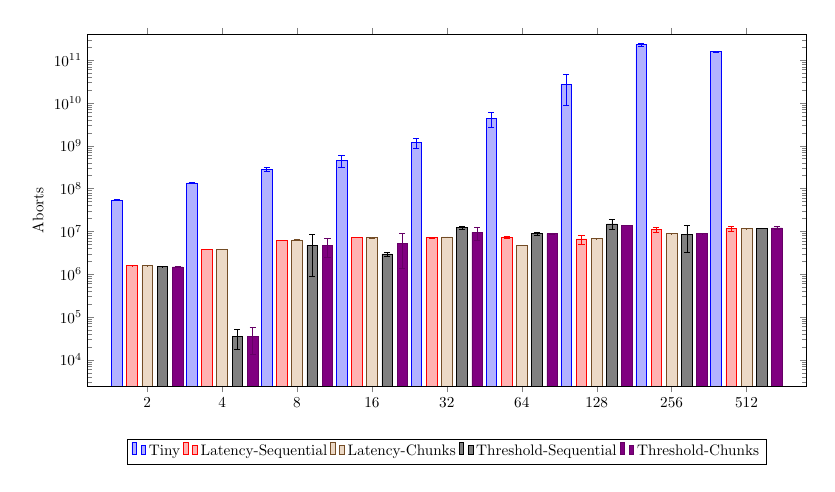
\begin{tikzpicture}[scale=0.55, baseline]
        \begin{axis}[
            ymode=log,
            width=1.5 \linewidth,
            height=0.8 \linewidth,
            %media de tempo intruder
            ybar=3pt,
            %enlargelimits=0.10,
            legend style={at={(0.5,-0.15)}, anchor=north, legend columns=-1},
            ylabel=Aborts,
            symbolic x coords={1, 2, 4, 8, 16, 32, 64, 128, 256, 512},
            xtick=data,
            ymin=0,
            ymax=400000000000,
            bar width=7pt,
            % nodes near coords,
            nodes near coords align={vertical},
        ]
        \addplot+[error bars,y dir=both, y explicit] coordinates {
            (1,0.0)+-(1,0.0) (2,53805739.2)+-(2,945974.4856792702) (4,136025541.2)+-(4,4837342.13) (8,281305083.6)+-(8,28618515.67361887) (16,455944205.2)+-(16,138166587.07) (32,1205121875.2)+-(32,315403375.80832976) (64,4297295036.4)+-(64,1609418223.03) (128,27371816768.6)+-(128,18399453268.002537) (256,230017372308.6)+-(256,19982225506.96) (512,156775482845.2)+-(512,5418181512.20) 
        };
        \addplot+[error bars,y dir=both, y explicit] coordinates {
            (1,0.0)+-(1,0.0) (2,1580633.2)+-(2,8478.500749542929) (4,3800972.6)+-(4,20650.110223434644) (8,6149664.4)+-(8,75882.93103880476) (16,7207458.2)+-(16,106075.91092684522) (32,7097792.4)+-(32,149914.3555148739) (64,7245601.6)+-(64,297306.3815181907) (128,6626592.6)+-(128,1601916.1098185633) (256,11035923.666666666)+-(256,1354186.7993902795) (512,11463741.25)+-(512,1422857.6912357355)
        };
        \addplot+[error bars,y dir=both, y explicit] coordinates {
             (1,0.0)+-(1,0.0) (2,1586885.6)+-(2,17013.20809959133) (4,3864768.25)+-(4,23733.99245149244) (8,6283745.6)+-(8,79485.5) (16,7192878.4)+-(16,178424.65) (32,7378729.9)+-(32,18573.11) (64,4723078.0)+-(64,3928.0) (128,6736182.0)+-(128,37123.3) (256,8828877.0)+-(256,12847.0) (512,11637482.0)+-(512,82034.0) 
        };
        \addplot+[error bars,y dir=both, y explicit] coordinates {
            (1,0.0)+-(1,0.0) (2,1502389.8)+-(2,8336.5398735266599) (4,34570.6)+-(4,17081.853735470282) (8,4673390.0)+-(8,3789634.775837482) (16,2964970.8)+-(16,290439.4272928145) (32,12301780.8)+-(32,1054972.452489657) (64,9002166.4)+-(64,735560.767845634) (128,14938022.8)+-(128,3727246.128412794) (256,8642330.0)+-(256,5465830.0) (512,11928378.731)+-(512,74928.0)
        };
        \addplot+[error bars,y dir=both, y explicit] coordinates {
            (1,0.0)+-(1,0.0) (2,1483981.3)+-(2,5287.71) (4,34983.38)+-(4,21305.7) (8,4728374.12)+-(8,2263748.1) (16,5260517.0)+-(16,3862894.25) (32,9462941.0)+-(32,3192100.38) (64,8837692.27)+-(64,384722.0) (128,13729279.5)+-(128,110344.5) (256,8874348.23)+-(256,63743.0) (512,11973628.0)+-(512,837874.02)
        };
        \legend {Tiny, Latency-Sequential, Latency-Chunks, Threshold-Sequential, Threshold-Chunks}
        \end{axis}
        \end{tikzpicture}
    }
    
    \caption{Aborts em NUMA variando o número de \emph{threads}.}
    \label{abort2}

\end{figure}

\chapter{Conclusão}
\label{chapter::conclusao}

Memória transacional (TM) fornece uma abstração para sincronização de threads em programas paralelos. Esteas podem ser implmentadas em hardware (HTM), software (STM) ou de forma hibrida com hardware e software. Este trabalho consentrace em aplicações de STM. Muitos estudos de STM apresentam escalonadores transacionais que focam em reduzir o número de conflitos por meio da serialização das transações reduzindo as threads ativas na aplicação ou bloqueando as transações conflitantes. Reduzir o número de conflitos se mostra eficiente para melhorar o desempenho, mas em arquiteturas multicore atuais com hierarquias de memória complexas também é importante considerar onde a posição de memória utilizada está localizada e por qual núcleo ela é acessada.

O entendimento da arquitetura utilizada, threads e dados é impotante para o desempenho, melhorando a localidade e reduzindo a latencia dos acessos à memória. As aplicações que utilizam STM fornecem oportunidades interessantes para entendimento da arquitetura e aplicação, pois em tempo de execução o STM fornece informações precisas sobre as áreas de memória que são compartilhadas entre threads, seus respectivos endereços e a intensidade com que cada endereço são acessados pelas threads. A partir do mapeamento destas informações este trabalhor desenvolveu um escalonador NUMA-Aware que permite a migração de threads entre as filas de execução.

A principal contribuição desta dissertação é um escalonador de STM, entitulado~\emph{LTMS} e apresentado em~\ref{chapter::ltms}, que adquira conhecimento sobre a arquitetura utilizada e suaa aplicaçã0, este conhecimento é gerado em tempo de execução por meio da colta de dados das threads e suas transações. Este escalonador fornece um mecanismo de distribuição inicial de threads, criação de filas, e migração de threads conflitantes entre as filas existentes. Este mecanismo busca otimizar o desempenhe de aplicações paralelas, reduzindo conflitos repetidos por meio da migração de threads agrupandoas as threads conflitantes na mesma filas. Para o desenvolvimento deste escalonador foi apresentada três etapas que temos como contribuções individuais do trabalho.

A etapa de inicialização contribui com um sistema de filas individuais para os núcleos, apresentado em~\ref{inicializacao}, na qual para executar a distribuição das threads entre estas filas podemos utilizar diferentes heuristicas para estudos, este trabalho apresentou duas heurísticas de distribuições. Estas heurísticas buscam distribuir inicialmente estas threads entre as filas disponiveis entender o comportamento do número inicial de conflitos existentes na aplicação e comportamento do acesso à memória.

Em tempo de execução o escalonador contribui com um mecanismo para coleta de dados da STM, apresentado em~\ref{coleta}, onde são montados duas matrizes uma de comunicação e uma de endereços. A matriz de comunicação fornece insumos sobre a quantidade de acessos aos endereços em comum entre threads. A matriz de endereços apresenta o endereço em comum mais acessado entre duas threads. Alem destas matrizes, são coletadas informações sobre a latencia de acesso à memória entre os nodos disponiveis na arquitetura e a quantidade de abortes e commites que ocorreram em cada trhead. Estas informações são insumos para compreender a arquitetura e a aplicação e são fundamentais para tomada de decisão na etapa de migração de threads do escalonador.

A ultima contribuição deste trabalho está em um sistema de migração de threads, apresentado em~\ref{migracao}, que é ativo apenas após a ocorrencia de um abort da aplicação. O escalonador identifica a thread que gerou o abort, e com base nas informações preveamente coletadas decide identifica para qual fila deve migrar está thread. O escalonador tem como base migrar a thread para uma fila na qual exista uma thread com maior número de acessos em comum à memória. Para tomada de decisão, se uma thread deve ou não ser migrada, é possivel utilizar diferentes heurística para estudo, nesta dissertação foi utilizada duas heurísticas. A primeira baseiase na relação entre abort e commit, quando está relação fica acima de um valor pré definido temos um indicativo de uma aplicação com alto indice de conflitos e o escalonador efetua a migração com intuido de reduzir os conflitos na aplicação, para identificar o valor limiar utilizado neste trabalho foram executados testes onde chegamos ao limiar de 0.8, que indica que com 80\% de abortes a thread deve ser migrada. A segunda heurística utiliza o custo da latencia no acesso à memória como parametro para efetuar a migração, onde se a fila atual que o thread executa possuir latencia maior que a fila para qual desejamos migrar o escalonador efetua a migração, está heurística busca reduzir o custo de latencia gasto na aplicação.

O escalonador foi desenvolvido sobre a biblioteca de STM TinySTM, e foram executados testes junto do conjundo de benchmarks STMAP, os exeperimentos foram rodados com o escalonador com ambas configurações de heuristicas desenvolvidas, como apresentado em~\ref{chapter::experimentos}, e comparados com a biblioteca original de TinySTM. Ambas as configurações de heuristicas apresentaram um desempenho de tempo melhor e número de conflitos menores que a TinySTM para maioria dos benchmarks testados. Concluímos que as aplicações ... \todo{concluir}

\section{\textbf{Trabalhos futuros}}

A pesquisa apresentada neste trabalho pode ser estendida das seguintes formas:

\begin{itemize}
	\item \emph{Novas heuristicas de distribuição}: O LTMS permite explorar distintas heuriticas de distribuição de threads ao inicializar a aplicação. Com isto é impotante avançarmos nos estudos para explorar diferentes formas de distribuição e comparalas. As distintas caracteristicas entre as heuristicas de distribuição podem ser exploradas em tralhos futuros.  

	\item \emph{Heuristica de migração hibrida}: O LTMS permite aplicar duas heuriticas de migração, uma com foco no indice de contenção e outra com foco na latencia de acesso à memória, mas o escalonador permite que estas heuristicas possam ser utilizadas juntas para aperfeiçoar o sistema de migração, buscando a redução da contenção e otimização do acesso à memória para reduzir a latencia da aplicação. 

	\item \emph{Impacto energetio dos escalonadore de STM}: Os trabalhos atuais focam no impacto que os escalonadores possuem sobre o desempenho de tempo e redução de conflitos. Um aspecto a ser abordado em trabalhos futuros pode ser o impacto que escalonador com consiencia da arquitetura, como o LTMS, possuem em relação ao custo energetico em relação a outros escalonadore.
\end{itemize}

O escalonado LTMS, desenvolvido nesta dissertação, pode ser estendido permitindo que estas caracteristicas sejam avaliadas em trabalhos futuros. Assim, podemos seguir com o desenvolvimento do LTMS contribuindo e explorando outros aspectos da área.

\bibliographystyle{abnt}
\bibliography{bibliografia} 

% Apêndices (Opcional) - Material produzido pelo autor
% \apendices
% \chapter{Um Apêndice}

% Anexos (Opcional) - Material produzido por outro
% \anexos
% \chapter{Um Anexo}

% \chapter{Outro Anexo}

% Faz a capa do CDROM
% \makecover

\end{document}

